\chapter{Evaluation}%
\label{cha:evaluation}

In this chapter, Whisker will be evaluated.
We will conduct three experiments to answer the following research questions:

{
    \parspace

    \centering
    \begin{minipage}{.9\textwidth}
        \textbf{RQ1: Can automated testing for Scratch produce test results that match the results of manual grading?}
        \parspace

        \textbf{RQ2: How flaky are automated tests for Scratch?}
        \parspace

        \textbf{RQ3: What statement coverage can be achieved by controlling Scratch programs with automatically generated input?}
        \parspace

        \textbf{RQ4: Does the testing process slow down the program under test?}
    \end{minipage}

    \parspace
}


\noindent In the first experiment, we will execute three different test suites on a set of Scratch projects
and determine the accuracy of our test results and the flakiness of our test suites.
For the second experiment, we will run a variety of projects with automated input generation
to find out how much of Scratch programs can be reached by automatically generated input.
Finally, in the third experiment we will measure execution times
to check if the testing process slows down the program under test.
\parspace

Section~\ref{sec:experimental_setup} describes the programs under test as well as the test suites we will use for the evaluation.
It also describes the software and hardware of our testing setup.
Then, Sections~\ref{sec:rq1}, \ref{sec:rq2}, \ref{sec:rq3}, and \ref{sec:rq4} each describe the results to one research question.
Each of the sections describes the experiment we conducted and the indicators we used
to answer the respective question.
Afterwards, we discuss the results in Section~\ref{sec:discussion}.
Finally, Section~\ref{sec:threats_to_validity} points out and discusses possible threats to validity.%
\parspace

The evaluation data will be available at \url{https://github.com/marvinkreis/bachelor-thesis/}.

\section{Experimental Setup}
\label{sec:experimental_setup}

\subsection{Testing Environment}

Figure~\ref{tab:evaluation_setup} lists the software and hardware we used to execute test suites on Scratch programs.
We used Whisker's web interface, which we described in Section~\ref{sec:testing_environment}, for this purpose.
All test executions were performed on the same machine.
For two parts of the evaluation,
specifically to measure execution time and to measure coverage over time,
we used slightly modified versions of Whisker as well as its GUI.

\begin{table}[htpb]
    \centering
    \scriptsize \tt
    \begin{tabular}{ll}
        \toprule
        Whisker     & Whisker 1.0 \\
        Scratch VM  & scratch-vm 0.2.0-prerelease.20181108204010 \\
        Web Browser & Chrome 70.0.3538.110 (64-Bit) \\
        JavaScript  & V8 7.0.276.40 \\
        OS          & Windows 8.1 Version 6.3 (Build 9600) \\
        CPU         & Intel Core i5 4670 (4 x  3.40 GHz) \\
        GPU         & Nvidia GeForce GTX 1080 \\
        RAM         & 8GB DDR3-1600 \\
        \bottomrule
    \end{tabular}
    \caption{Software and hardware used for evaluation}
    \label{tab:evaluation_setup}
\end{table}

\subsection{Projects Under Test}

This section will list the Scratch projects we used to evaluate Whisker and explain why we chose these projects.

\subsubsection{(P1) Catching Game}

The first set of Scratch projects consists of 37 student implementations of a simple catching game.
The projects originate from a voluntary Scratch workshop for sixth and seventh grade students~\cite{keller}.
In this workshop, students were introduced to Scratch through several small exercises,
% familiarized themselves with Scratch
building up to the final and most complex exercise to develop the aforementioned catching game.
Students were given a Scratch project as a template to fill with their implementation.
\parspace

In this game, apples and bananas periodically fall from random positions at the top of the screen.
The player earns points by catching these fruits with a bowl at the bottom of the screen,
which is controlled with the left and right arrow keys.
The game ends when 30 seconds have passed or if an apple touches the ground (a game over).
A screenshot of the sample implementation of this program can be seen in Figure~\ref{fig:screenshot_of_the_sample_implementation}
and a summary of the program specification from the assignment is included in Table~\ref{tab:project_specification}.
Additionally, the full task description from the workshop (in german) may be found in Figure~\ref{fig:catching_game_task_description} in the appendix.
\parspace

\begin{figure}[htpb]
    \centering
    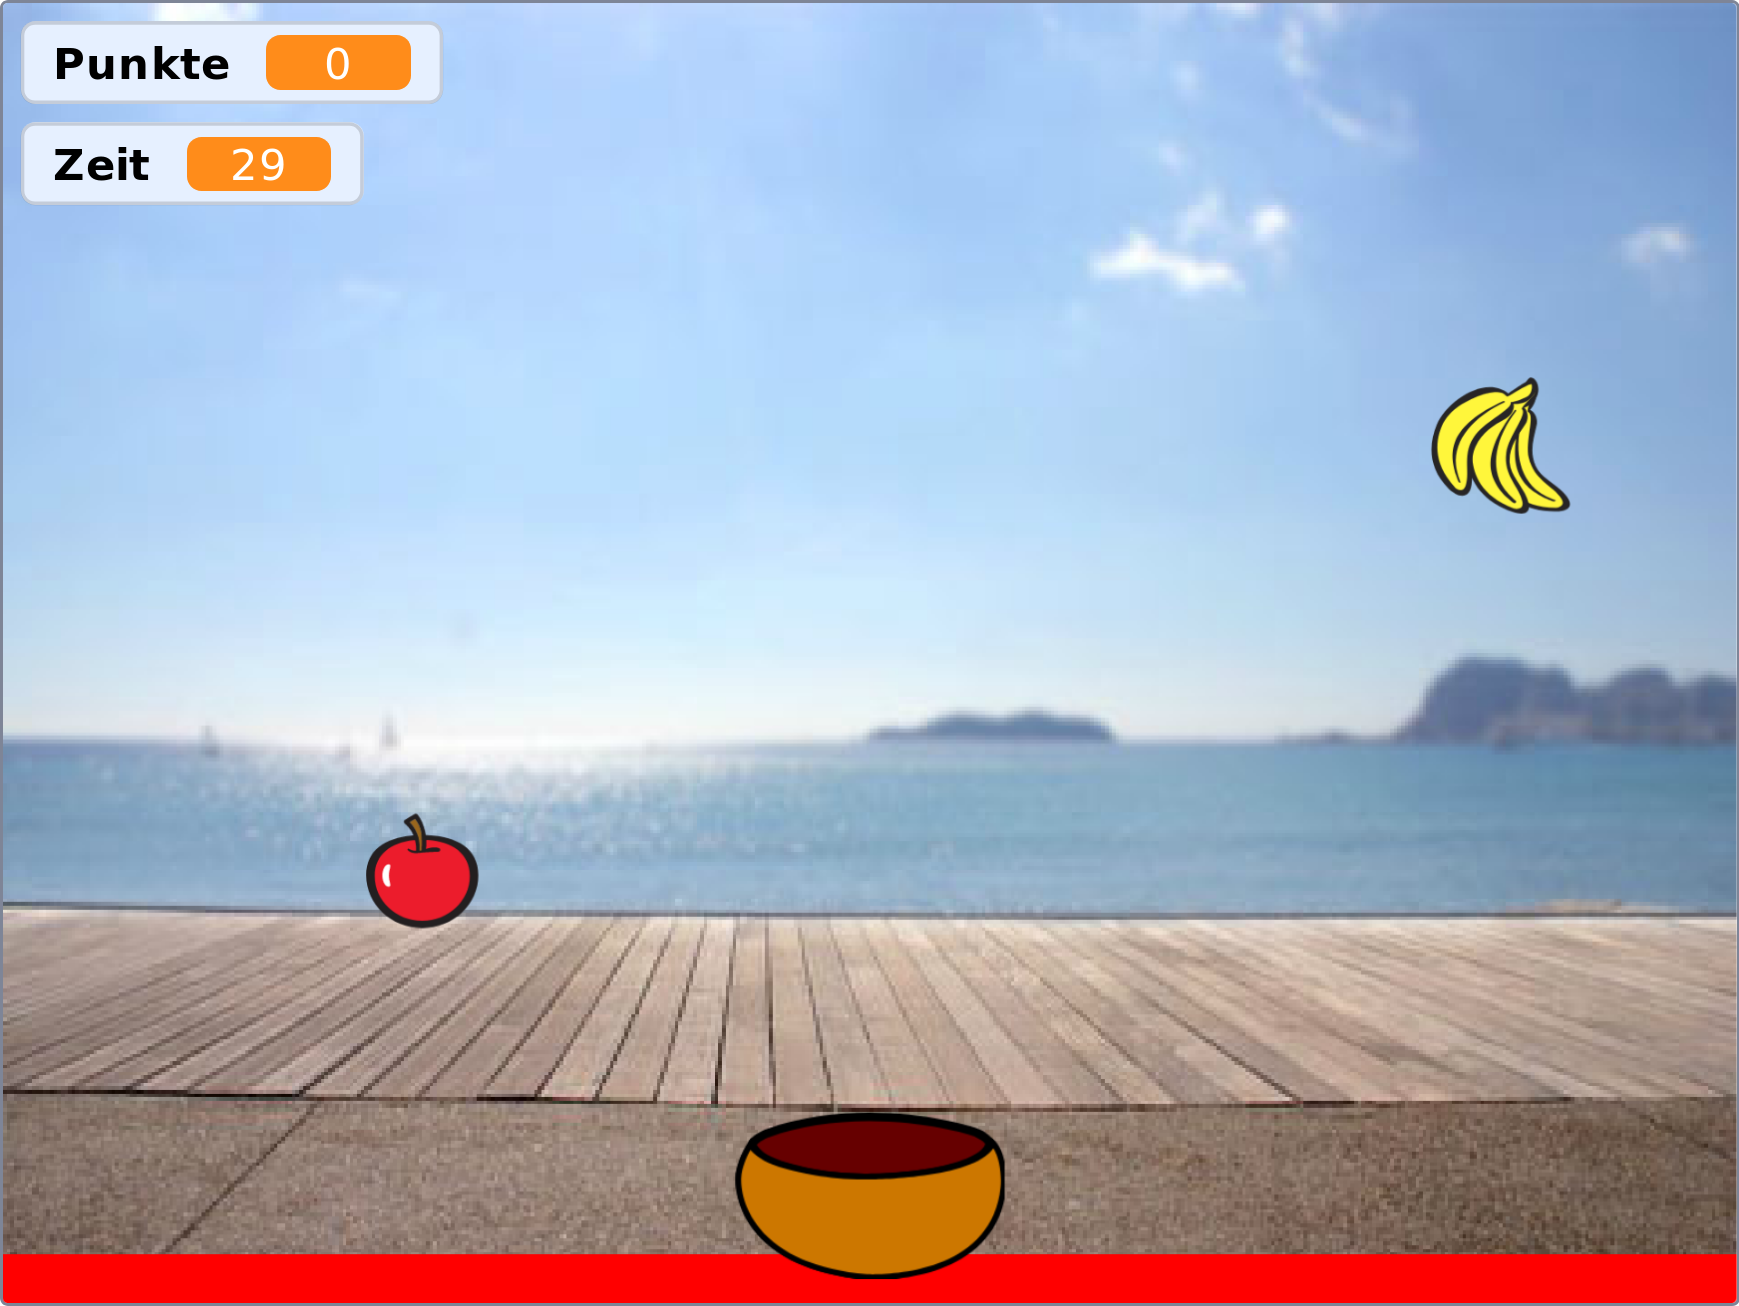
\includegraphics[width=0.30\textwidth]{scratch-stage}
    \caption{Screenshot of the sample implementation}
    \label{fig:screenshot_of_the_sample_implementation}
\end{figure}

The Scratch projects in this set were manually evaluated and scored using a point-based grading scheme in the range of $[0, 30]$.
This enables us to determine the quality of our test results by using the manually assigned scores as ground truth,
and comparing the results of automated testing to them.
Table~\ref{tab:manual_scores_and_test_passes_of_each_project} contains the manual scores for each project and
Table~\ref{tab:manual_grading_scheme} shows the grading scheme used to determine the scores.
\parspace

We use these projects to evaluate the accuracy of our testing approaches.
The projects are very suitable for this task because of two reasons.
Firstly, there exists a relatively precise specification for the programs,
which enables us to test the implementations according to this specification.
And secondly, the student solutions are of varying degrees of quality,
which is desirable for the evaluation,
because we can analyze a wide range of different outcomes.
% The projects are suitable for this evaluation because of two reasons.
% Firstly, the task description specifies the program well, which enables us to write automated tests according to the specification.
% Secondly, the student solutions are of varying degrees of quality,
% which is desirable, so automated tests produce a range of different outcomes.
% However, testing these projects has also revealed some challenges.
% For one thing, these projects were never meant to be subject to automated testing.
% Therefore, some details, mainly the usage of clones,
% are not part of the task specification, which complicates testing,
% since tests have to consider multiple options.
% Additionally, the game over state, that the program enters,
% when an apple touches the ground, also makes automated testing more difficult.
\parspace

However, since the Scratch programs were not written for the purpose of automated testing,
some of the projects were unusable for our evaluation.
Therefore, we excluded $6$ of the 37 projects in our statistics.
Table~\ref{tab:excluded_projects} shows the excluded projects together with the reasons for excluding them.
% The projects are named K6\_S01 through K6\_S33 for 6th grade student solutions
% and K7\_S02 through K7\_S27 for 7th grade student solutions respectively (with many numbers being skipped).
Most of the projects were excluded because they don't start properly.
% This seems to be a common problem, since Scratch runs programs from where they left off in the last run.
% But to get consistent test results, we have to establish the same situation before every test case,
% which we do by loading the project.
Some of the projects start with a key press instead of the green flag,
others go game over when they are started the first time, but work in subsequent runs.
Since the specification did not actually specify that the programs have to start with the green flag,
the manual scoring ignores these problems, but our tests don't.
% But the program not starting correctly is technically a fault in the implementation, so low test scores are correct for these projects.
Hence, these projects would create a discrepancy between manual scores and test results,
which only exists due to the difference in scoring systems.
We believe the statistics convey our results more clearly without these projects.

\begin{table}[htpb]
    \centering
    \scriptsize
    \begin{tabular}{lp{10.5cm}}
        \toprule
        Project & Reason                                                                           \\
        \midrule
        \multicolumn{2}{l}{\textbf{Detected through test reports}}                                 \\
      % K6\_S12 & Deleted variable from template: ''Zeit''                                         \\
      % K6\_S17 & Renamed variable from template: ''Punkte'' to ''Bunkte''                         \\
      % K7\_S24 & Deleted variable from template: ''Zeit''                                         \\
      % K7\_S27 & Renamed sprite from template: ''Bowl'' to ''Figur2''                             \\
        K7\_S07 & Resets all sprite positions when the "a" key is pressed.
                  Automated test input generation picks up on this and
                  simulates presses on the "a" key.                                                \\[1.4\bigskipamount]

        \multicolumn{2}{l}{\textbf{Detected through zero statement coverage}}                      \\
        K6\_S01 & Starts on up arrow key press instead of green flag.                              \\
        K6\_S06 & Starts on space key press instead of green flag.                                 \\
        K6\_S14 & Starts on space key press instead of green flag.                                 \\[\medskipamount]

        \multicolumn{2}{l}{\textbf{Detected manually}}                                             \\
        K6\_S20 & Goes game over when green flag is pressed the first time.                        \\
        K7\_S18 & Goes game over on start unless sprites are re-positioned manually in the editor. \\
        \bottomrule
    \end{tabular}
    \caption{Excluded projects from P1 and the reasons for their exclusion}
    \label{tab:excluded_projects}
\end{table}

\subsubsection{(P2) Code Club Projects}

The second set of Scratch projects consists of sample solutions to 24 of Code Club's~\cite{codeclub} Scratch exercises.
Code Club offers free coding projects and step by step guides for programming beginners.
For each project, a sample solution is provided by a volunteer.
\parspace

We use these projects to evaluate Whisker's automated input generation.
The projects work well for this task since they implement a variety of different programs with different input methods.
Table~\ref{tab:code_club_stats} displays the input methods the projects use.
We chose the sample solutions of the exercises since measuring coverage on working implementation will yield better results.
Broken implementations are more likely to have unreachable code,
because some code might depend on a feature that is not implemented correctly.

\begin{table}[htpb]
    \centering
    \scriptsize
    \scalebox{.90}{
    \begin{tabular}{l|lll|lll}
        \toprule
        Project & \rotatebox{90}{\texttt{\#} Sprites} & \rotatebox{90}{\texttt{\#} Scripts} & \rotatebox{90}{\texttt{\#} Blocks}
                & \rotatebox{90}{Mouse} & \rotatebox{90}{Keyboard} & \rotatebox{90}{Ask-Answer} \\
        \midrule
        Archery & 2 & 3 & 21 & \xmark & \cmark & \xmark \\
        Balloons & 2 & 4 & 26 & \cmark & \xmark & \xmark \\
        Beat The Goalie & 3 & 6 & 30 & \xmark & \cmark & \xmark \\
        Boat Race & 3 & 3 & 27 & \cmark & \xmark & \xmark \\
        Brain Game & 4 & 19 & 76 & \cmark & \xmark & \cmark \\
        Catch The Dots & 5 & 11 & 82 & \xmark & \cmark & \xmark \\
        Chat Bot & 2 & 2 & 26 & \cmark & \xmark & \cmark \\
        Clone Wars & 7 & 17 & 76 & \xmark & \cmark & \xmark \\
        Create Your Own World & 13 & 26 & 165 & \xmark & \cmark & \xmark \\
        Dodgeball & 5 & 10 & 78 & \xmark & \cmark & \xmark \\
        Ghostbusters & 5 & 11 & 58 & \cmark & \xmark & \xmark \\
        Green Your City & 7 & 8 & 52 & \xmark & \cmark & \xmark \\
        Lost In Space & 6 & 4 & 24 & \xmark & \xmark & \xmark \\
        Memory & 6 & 11 & 58 & \cmark & \xmark & \cmark \\
        Moonhack Scratch 2017 & 3 & 4 & 27 & \xmark & \cmark & \xmark \\
        Poetry Generator & 4 & 2 & 18 & \cmark & \xmark & \cmark \\
        Rock Band & 5 & 6 & 18 & \cmark & \xmark & \xmark \\
        Snowball Fight & 4 & 7 & 37 & \xmark & \cmark & \xmark \\
        Space Junk & 8 & 13 & 68 & \xmark & \cmark & \xmark \\
        Sprint & 5 & 9 & 78 & \xmark & \cmark & \xmark \\
        Synchronised Swimming & 2 & 7 & 23 & \xmark & \cmark & \xmark \\
        Tech Toys & 9 & 5 & 25 & \cmark & \cmark & \xmark \\
        Username Generator & 3 & 2 & 5 & \cmark & \xmark & \xmark \\
        Paint Box & 9 & 14 & 42 & \cmark & \xmark & \xmark \\
        \bottomrule
    \end{tabular}
    }
    \caption{Block counts and input methods of the Code Club projects (P2)}
    \label{tab:code_club_stats}
\end{table}

\subsection{Test Suites}

The set of catching game projects (P1) will be tested with three different test suites
in order to analyze the quality of their test results.
Table~\ref{tab:project_specification} lists which part of the specification is covered by each test suite.
Additionally, the number of tests or constraints, and the size of the test suite measured in source lines of code (SLOC),
can be found in Table~\ref{tab:test_suite_statistics}.
In this section, we will describe each of the test suites.

\begin{table}[htpb]
    \centering
    \scriptsize
    \begin{tabular}{rlrlr}
        \toprule
        Test Suite & Type       & \texttt{\#}Tests / \texttt{\#}Constraints & SLOC \\
        \midrule
        T1         & Normal     & 28 Tests                                  &  852 \\
        T2         & Constraint & 26 Constraints                            &  620 \\
        T3         & Constraint & 26 Constraints                            &  618 \\
        \bottomrule
    \end{tabular}
    \caption{Number of tests and source lines of code per test suite}
    \label{tab:test_suite_statistics}
\end{table}

\begin{table}[htpb]
    \centering
    \scriptsize
    \begin{tabular}{rl|cr|cr|cr}
        \toprule
        \texttt{\#} & Specification  & \multicolumn{6}{c}{Covered?, Test Number} \\
                                    && \multicolumn{2}{l|}{T1} & \multicolumn{2}{l|}{T2} & \multicolumn{2}{l}{T3}    \\
        \midrule
           & \textbf{Initialization} &&&&&&\\
         1 & Timer starts at 30 seconds and score starts at 0                          & \cmark & 1  & \cmark & 1  & \cmark & 1  \\
         2 & Bowl starts at $X = 0$ / $Y = -145$                                       & \cmark & 2  & \cmark & 2  & \cmark & 2  \\
         3 & Fruits have a size of 50\%                                                & \cmark & 3  & \cmark & 3  & \cmark & 3  \\[\medskipamount]
           & \textbf{Bowl Movement} &&&&&&\\
         4 & Bowl moves left/right when the corresponding arrow key is pressed         & \cmark & 4  & \cmark & 4  & \cmark & 4  \\
         5 & Bowl can only move horizontally with a speed of 10                        & \cmark & 5  & \cmark & 5  & \cmark & 5  \\[\medskipamount]
           & \textbf{Fruit Falling} &&&&&&\\
         6 & Apples fall down                                                          & \cmark & 6  & \cmark & 6  & \cmark & 6  \\
         7 & Apples fall in a straight line with a speed of -5                         & \cmark & 7  & \cmark & 7  & \cmark & 7  \\
         8 & Bananas fall down                                                         & \cmark & 8  & \cmark & 8  & \cmark & 8  \\
         9 & Bananas fall in a straight line with a speed of -7                        & \cmark & 9  & \cmark & 9  & \cmark & 9  \\[\medskipamount]
           & \textbf{Fruit Spawn} &&&&&&\\
        10 & Apples spawn again at the top of the screen after touching the bowl       & \cmark & 10 & \cmark & 10 & \cmark & 10 \\
        11 & Apples spawn at random $X$ positions                                      & \cmark & 11 & \cmark & 11 & \cmark & 11 \\
        12 & Apples spawn at $Y = 170$                                                 & \cmark & 12 & \cmark & 12 & \cmark & 12 \\
        13 & Bananas spawn again at the top after touching the bowl or the ground      & \cmark & 13 & \cmark & 13 & \cmark & 13 \\
        14 & Bananas spawn at random $X$ positions                                     & \cmark & 14 & \cmark & 14 & \cmark & 14 \\
        15 & Bananas spawn at $Y = 170$                                                & \cmark & 15 & \cmark & 15 & \cmark & 15 \\
        16 & Only one apple must fall down at a time                                   & \cmark & 16 & \cmark & 16 & \cmark & 16 \\
        17 & Only one banana must fall down at a time                                  & \cmark & 17 & \cmark & 17 & \cmark & 17 \\
        18 & Banana must wait for a second before falling down in the beginning        & \cmark & 18 & \cmark & 18 & \cmark & 18 \\
        19 & Banana must wait for a second before falling down after displaying ''-8'' & \cmark & 19 & \cmark & 19 & \cmark & 19 \\[\medskipamount]
           & \textbf{Fruit Interaction} &&&&&&\\
        20 & Apple gives 5 points when it touches the bowl                             & \cmark & 20 & \cmark & 20 & \cmark & 20 \\
        21 & Game over when the apple touches the ground                               & \cmark & 21 & \xmark &    & \cmark & 21 \\
        22 & Apple displays ''Game Over!'' message when it touches the ground          & \cmark & 22 & \xmark &    & \cmark & 22 \\
        23 & Banana gives 8 points when it touches the bowl                            & \cmark & 23 & \cmark & 21 & \cmark & 23 \\
        24 & Banana subtracts 8 points when it touches the ground                      & \cmark & 24 & \cmark & 22 & \cmark & 24 \\
        25 & Banana displays ''-8'' message when it touches the ground                 & \cmark & 25 & \cmark & 23 & \cmark & 25 \\[\medskipamount]
           & \textbf{Timer} &&&&&&\\
        26 & Timer ticks down                                                          & \cmark & 26 & \cmark & 24 & \cmark & 26 \\
        27 & Game stops when timer reaches 0                                           & \cmark & 27 & \cmark & 25 & \xmark &    \\
        28 & Bowl must display ''Ende!'' message when timer reaches 0                  & \cmark & 28 & \cmark & 26 & \xmark &    \\
        \bottomrule
    \end{tabular}

    \caption{Project specification and each test suite's coverage of the specification}
    \label{tab:project_specification}
\end{table}

\subsubsection{(T1) Normal Test Suite}

This test suite follows an ordinary testing approach.
Each test case runs the program once in order to check one part of the specification,
mostly without the use of constraints.
Tests simulate inputs deliberately and mostly perform assertions between runs of the program.
% Listing~\ref{lst:example_test_case_normal} shows a shortened example of a simple test case from this test suite.
% which tests the user interaction with the bowl sprite.
The test suite encompasses 28 test cases, which correspond to the specification in Table~\ref{tab:project_specification}.
\parspace

% \begin{listing}[htpb]
%     \centering
%     \begin{minipage}{.70\textwidth}
%         \begin{minted}[autogobble, breaklines, linenos, fontsize=\scriptsize, framesep=2mm, frame=lines]{javascript}
%             const testMoveBowl = async function (t, testDetails = false) {
%                 const {bowl} = getSpritesAndVariables(t, ['bowl']);
%                 let bowlX;
%
%                 /* Give the program some time to initialize. */
%                 await t.runForTime(250);
%
%                 /* Test movement when no key is pressed. */
%                 bowlX = bowl.x;
%                 await t.runForTime(250);
%                 t.assert.equal(bowl.x, bowlX,
%                     'Bowl must not move when no key is pressed.');
%
%                 /* Test movement when left arrow key is pressed. */
%                 t.inputImmediate({
%                     device: 'keyboard',
%                     key: 'left arrow',
%                     isDown: true,
%                     duration: 50
%                 });
%                 bowlX = bowl.x;
%                 await t.runForTime(250);
%                 t.assert.less(bowl.x, bowlX,
%                     'Bowl must move to the left when left arrow key is pressed.');
%
%                 /* Test movement when right arrow key is pressed. */
%                 ...
%             };
%         \end{minted}
%     \end{minipage}
%
%     \caption{Shortened example test case from test suite T1}
%     \label{lst:example_test_case_normal}
% \end{listing}

For many test cases, the catching game has to be played without letting an apple touch the ground for a period of time.
In order to accomplish this, we implemented a function
that takes the x coordinates of the apple and bowl sprites,
and simulates arrow key presses to move the bowl towards the apple's position.
This function, as well as a usage example, are shown in Listing~\ref{lst:simulating_catching_game}.

\begin{listing}[htpb]
    \centering
    \begin{minipage}{.85\textwidth}
        \begin{minted}[autogobble, breaklines, linenos, fontsize=\tiny, framesep=2mm, frame=lines]{javascript}
            const followSprite = function (t, bowlX, spriteX) {
                /* Stop if the bowl is near enough. */
                if (Math.abs(bowlX - spriteX) <= 10) {
                    t.inputImmediate({device: 'keyboard', key: 'left arrow',  isDown: false});
                    t.inputImmediate({device: 'keyboard', key: 'right arrow', isDown: false});

                } else if (bowlX > spriteX) {
                    t.inputImmediate({device: 'keyboard', key: 'right arrow', isDown: false});
                    t.inputImmediate({device: 'keyboard', key: 'left arrow',  isDown: true});

                    /* Trick "when key pressed" hats to fire by letting go of the key and immediately pressing it again. */
                    t.inputImmediate({device: 'keyboard', key: 'left arrow',  isDown: false});
                    t.inputImmediate({device: 'keyboard', key: 'left arrow',  isDown: true});

                } else if (bowlX < spriteX) {
                    t.inputImmediate({device: 'keyboard', key: 'left arrow',  isDown: false});
                    t.inputImmediate({device: 'keyboard', key: 'right arrow', isDown: true});

                    /* Trick "when key pressed" hats to fire by letting go of the key and immediately pressing it again. */
                    t.inputImmediate({device: 'keyboard', key: 'right arrow', isDown: false});
                    t.inputImmediate({device: 'keyboard', key: 'right arrow', isDown: true});
                }
            };

            const testSomething = function (t) {
                ...
                /* Catch apples with the bowl during runs. */
                t.addCallback(() => {
                    apple = getNewestClone(apple);
                    followSprite(t, bowl.x, apple.x);
                });
                ...
            };
        \end{minted}
    \end{minipage}

    \caption{Code for simulating arrow key presses for the catching game}
    \label{lst:simulating_catching_game}
\end{listing}

\subsubsection{(T2) Constraint Test Suite}

This test suite implements the constraint testing approach from Chapter~\ref{cha:using_constraints_for_flexible_test_inputs}.
With this test suite, we tried to test the program with only one execution in total.
Therefore, this test suite only has a single test case, which registers 26 constraints to check various parts of the specification
(corresponding to Table~\ref{tab:project_specification}).
\parspace

This test case deliberately simulates inputs with the goal of winning the game.
We use the same helper method as test suite T1 to simulate key presses depending on the bowl's and the apple's position.
Because of this, the bowl should always catch the apple in working implementations,
and the program should never go game over because of an apple touching the ground.
Therefore, we don't check the interaction between the apple sprite and the ground with this test suite.

\subsubsection{(T3) Random Input Test Suite}

This test suite uses 26 constraint, which are mostly the same T2's.
It uses Whisker's automated input generation to control the program with random inputs,
and resets the program multiple times in order to increase the likelihood of multiple apples getting caught in one of the runs.
But since it is nevertheless very unlikely to have the apple not touch the ground at all with random inputs,
we don't for check for a game over after 30 seconds, and only let the program run for 10 seconds a time.
We chose to reset the program 30 times during the test, resulting in an execution time of $30 \times 10s = 300s$.
Listing~\ref{lst:automated_input_random_tests} shows the exact configuration we used to simulate input for the test case.
We chose to simulate random inputs with a duration between $50\text{ms}$ and $100\text{ms}$ in an interval of $150\text{ms}$.
\parspace

\begin{listing}[htpb]
    \centering
    \begin{minipage}{.55\textwidth}
        \begin{javascriptcode}
            t.setRandomInputInterval(150);
            t.detectRandomInputs({duration: [50, 100]});
        \end{javascriptcode}
    \end{minipage}
    \caption{Code for automated input generation in test suite T3 (random input)}
    \label{lst:automated_input_random_tests}
\end{listing}

\section{RQ1: Accuracy of Test Results}
\label{sec:rq1}

In this section, we will answer the following research question:

\begin{center}\begin{minipage}{.9\textwidth}
    \textbf{RQ1: Can automated testing for Scratch produce test results that match the results of manual grading?}
\end{minipage}\end{center}

\noindent In order to answer this question,
we executed test suites T1-T3 on the catching game projects (P1) ten times,
and analyzed the results.
To be useful for grading,
test results have to indicate the same grades,
which one would assign the programs through manual assessment.
% Test outcomes also have to be consistent over multiple runs,
% since inconsistent results would lead to unfair grades.
% Therefore, we analyzed the correlation between the number of test passes and the manually assigned scores.
Intuitively, a higher score means that more tests (or constraints) should pass,
while a lower score should result in fewer test (or constraint) passes.
Therefore, we use the correlation between the number of test passes and the manual scores as an indicator.
We measure the correlation through Pearson's correlation coefficient, which is denoted as $r$.
$r$ can take on values in the range of $[-1, 1]$.
A high correlation coefficient indicates a strong relationship between two values,
while a low correlation coefficient indicates a weak relationship.
Usually, a value of $r \ge 0.5$ is considered to indicate a strong correlation.
Negative values indicate a reverse relationship, which is not relevant for our observations.

\paragraph{Null hypothesis ($H_0$):}
The number of test passes and the results of manual scoring only show a weak correlation or no correlation at all.
\vspace{-\medskipamount}
\paragraph{Alternative hypothesis ($H_1$):}
The number of test passes closely match manually assigned scores.
They have a strong correlation.

\subsubsection{Normal Test Suite (T1)}

Figure~\ref{fig:scatter_normal} compares each project's number of test passes of test suite T1 to its manual score.
Possible values for the manual scores are in the range of $[0, 30]$ and possible values for the number of test passes are in the range of $[0, 28]$.
The blue line displays the linear regression.
We can observe a strong correlation between the number of passing test cases and the manual scores,
with a correlation coefficient of $r = 0.893$ (p-value = 1.45e-11) for the first run and $r = 0.899$ (p-value = 6.59e-12) for the average number of passes over ten runs.
Except for few irregularities, the test results closely resemble the manually assigned scores.

\subsubsection{Constraint Test Suite (T2)}

Figure~\ref{fig:scatter_constraint} compares each project's number of passing constraints of test suite T2 to its manual score.
Possible values for the number of constraint passes are in the range of $[0, 26]$.
We can again observe a strong correlation between the two scores,
with a correlation coefficient of $r = 0.878$ (p-value = 9.06e-11) for the first run and $r = 0.889$ (p-value = 2.43e-11) for the average number of passes over ten runs.

\subsubsection{Random Input Test Suite (T3)}

Figure~\ref{fig:scatter_constraint} compares the constraint passes of test suite T3 to the manual scores.
Possible values for the number of constraint passes are in the range of $[0, 26]$.
The results indicate a strong correlation with a correlation coefficient of $r = 0.869$ (p-value = 2.39e-10) for the first run and $r = 0.882$ (p-value = 5.23e-11) for the average over ten runs.
\parspace

\noindent Each project's manual scores and number of test passes can be found in Table~\ref{tab:manual_scores_and_test_passes_of_each_project}.

\begin{figure}[htpb]
    \centering
    \begin{subfigure}{.85\textwidth}
        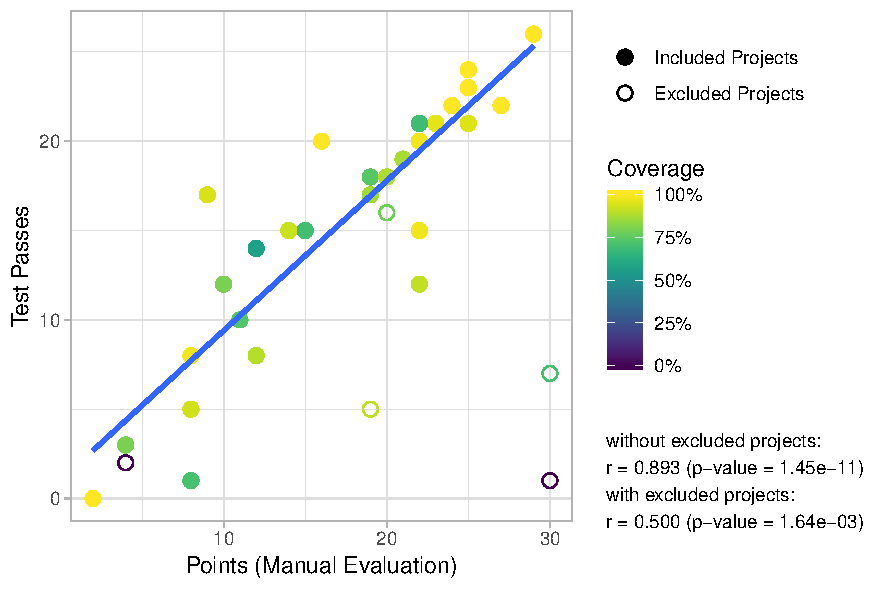
\includegraphics[width=\textwidth]{r/scatter-normal-1}
        \caption{First run}
        \label{fig:scatter_normal_1}
    \end{subfigure}

    \bigskip

    \begin{subfigure}{.85\textwidth}
        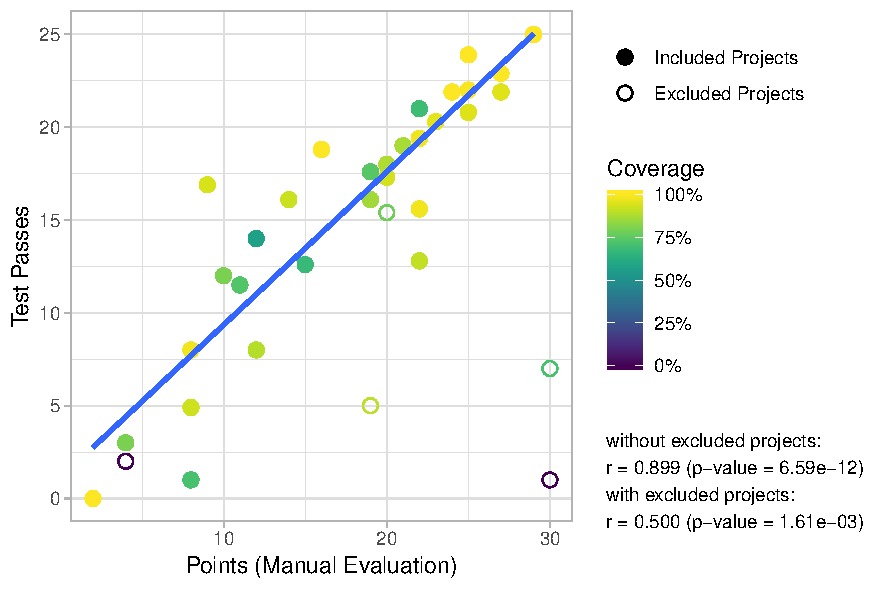
\includegraphics[width=\textwidth]{r/scatter-normal-avg}
        \caption{Average over ten runs}
        \label{fig:scatter_normal_avg}
    \end{subfigure}
    \caption{Comparison between test results of test suite T1 (normal) and manually assigned scores}
    \label{fig:scatter_normal}
\end{figure}

\begin{figure}[htpb]
    \centering
    \begin{subfigure}{.85\textwidth}
        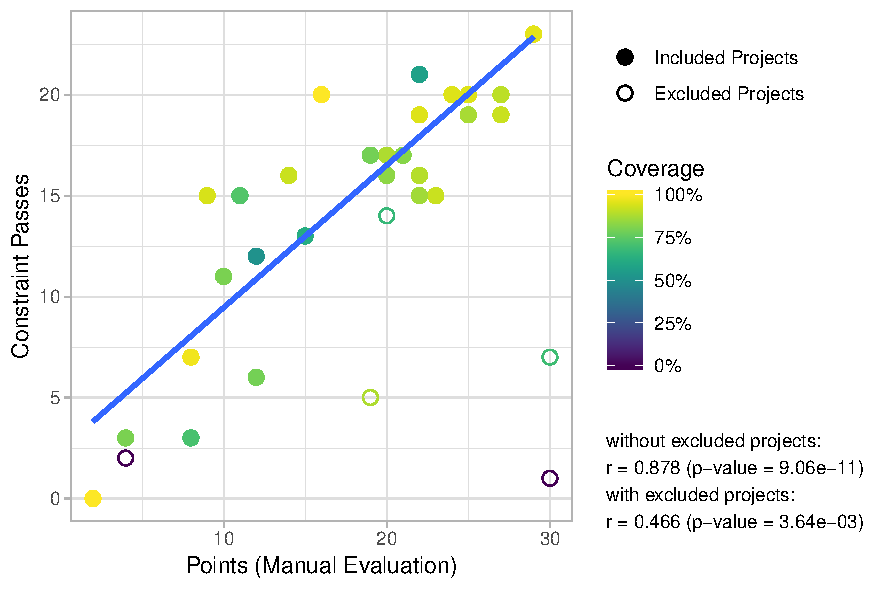
\includegraphics[width=\textwidth]{r/scatter-constraint-1}
        \caption{First run}
        \label{fig:scatter_constraint_1}
    \end{subfigure}

    \bigskip

    \begin{subfigure}{.85\textwidth}
        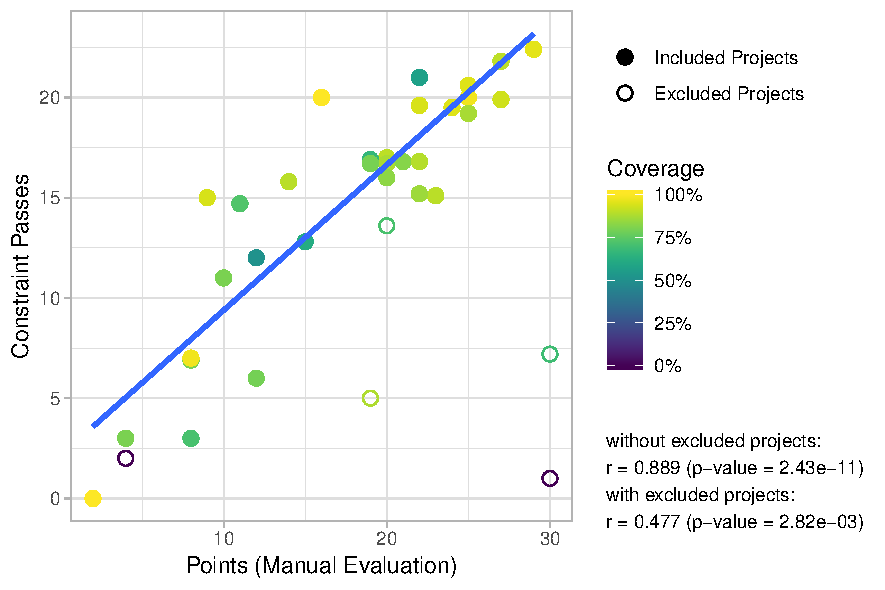
\includegraphics[width=\textwidth]{r/scatter-constraint-avg}
        \caption{Average over ten runs}
        \label{fig:scatter_constraint_avg}
    \end{subfigure}
    \caption{Comparison between test results of test suite T2 (constraint) and manually assigned scores}
    \label{fig:scatter_constraint}
\end{figure}

\begin{figure}[htpb]
    \centering
    \begin{subfigure}{.85\textwidth}
        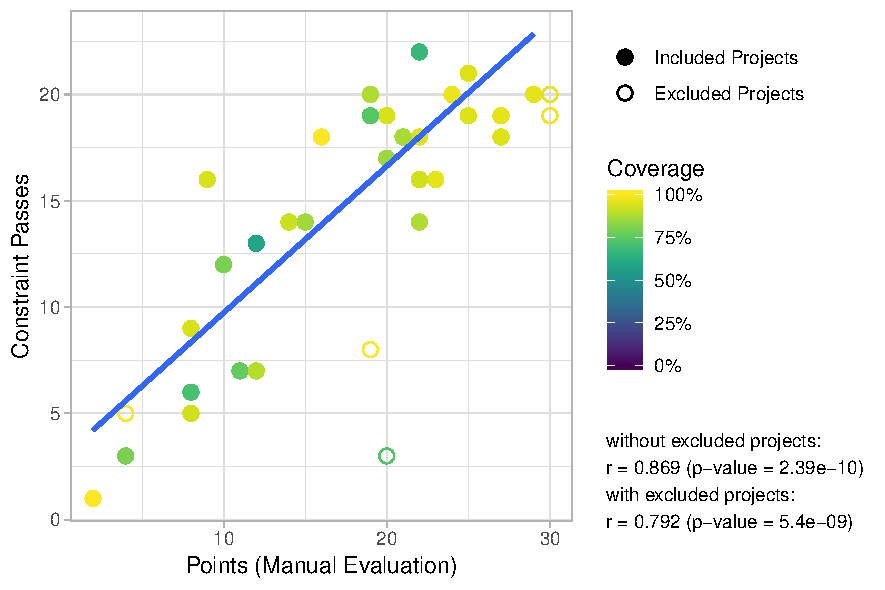
\includegraphics[width=\textwidth]{r/scatter-random-1}
        \caption{First run}
        \label{fig:scatter_random_1}
    \end{subfigure}

    \bigskip

    \begin{subfigure}{.85\textwidth}
        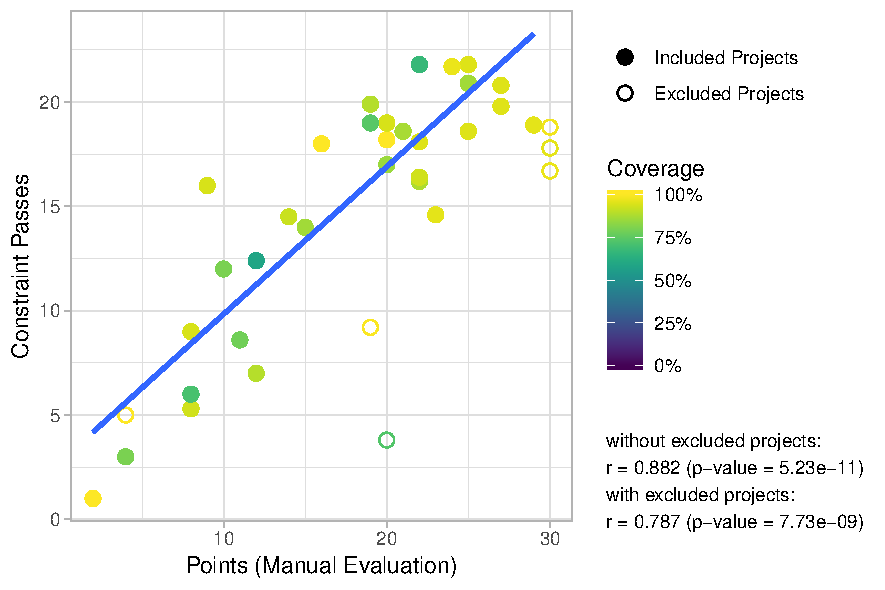
\includegraphics[width=\textwidth]{r/scatter-random-avg}
        \caption{Average over ten runs}
        \label{fig:scatter_random_avg}
    \end{subfigure}
    \caption{Comparison between test results of test suite T3 (random input) and manually assigned scores}
    \label{fig:scatter_random}
\end{figure}

\begin{table}[htpb]
    \centering
    \scriptsize
    \begin{tabular}{lc|r|rr|rr|rr}
        \toprule
        Project & Excl. & Points & T1 1st & T1 avg & T2 1st & T2 avg & T3 1st & T3 avg \\
        \midrule
        K6\_S01 & \cmark & 30 &  1 &  1.0 &  1 &  1.0 & 20 & 17.8 \\
        K6\_S02 & \xmark & 15 & 15 & 12.6 & 13 & 12.8 & 14 & 14.0 \\
        K6\_S03 & \xmark & 11 & 10 & 11.5 & 15 & 14.7 &  7 &  8.6 \\
        K6\_S05 & \xmark & 23 & 21 & 20.3 & 15 & 15.1 & 16 & 14.6 \\
        K6\_S06 & \cmark & 30 &  1 &  1.0 &  1 &  1.0 & 19 & 16.7 \\
        K6\_S10 & \xmark & 22 & 20 & 19.4 & 19 & 19.6 & 18 & 18.1 \\
        K6\_S11 & \xmark &  8 &  5 &  4.9 &  7 &  6.9 &  5 &  5.3 \\
        K6\_S13 & \xmark &  8 &  8 &  8.0 &  7 &  7.0 &  9 &  9.0 \\
        K6\_S14 & \cmark &  4 &  2 &  2.0 &  2 &  2.0 &  5 &  5.0 \\
        K6\_S15 & \xmark & 10 & 12 & 12.0 & 11 & 11.0 & 12 & 12.0 \\
        K6\_S16 & \xmark &  2 &  0 &  0.0 &  0 &  0.0 &  1 &  1.0 \\
        K6\_S18 & \xmark & 27 & 22 & 21.9 & 19 & 19.9 & 19 & 19.8 \\
        K6\_S19 & \xmark & 25 & 23 & 22.0 & 20 & 20.0 & 21 & 20.9 \\
        K6\_S20 & \cmark & 30 &  7 &  7.0 &  7 &  7.2 & 19 & 18.8 \\
        K6\_S27 & \xmark &  4 &  3 &  3.0 &  3 &  3.0 &  3 &  3.0 \\
        K6\_S29 & \xmark & 12 &  8 &  8.0 &  6 &  6.0 &  7 &  7.0 \\
        K6\_S30 & \xmark & 20 & 18 & 18.0 & 17 & 17.0 & 19 & 18.2 \\
        K6\_S31 & \xmark & 16 & 20 & 18.8 & 20 & 20.0 & 18 & 18.0 \\
        K6\_S33 & \xmark & 20 & 18 & 17.3 & 17 & 16.7 & 19 & 19.0 \\
        K7\_S02 & \xmark & 19 & 18 & 17.6 & 17 & 16.9 & 19 & 19.0 \\
        K7\_S03 & \xmark & 14 & 15 & 16.1 & 16 & 15.8 & 14 & 14.5 \\
        K7\_S04 & \xmark & 12 & 14 & 14.0 & 12 & 12.0 & 13 & 12.4 \\
        K7\_S05 & \xmark & 22 & 21 & 21.0 & 21 & 21.0 & 22 & 21.8 \\
        K7\_S06 & \xmark & 20 & 18 & 18.0 & 16 & 16.0 & 17 & 17.0 \\
        K7\_S07 & \cmark & 20 & 16 & 15.4 & 14 & 13.6 &  3 &  3.8 \\
        K7\_S08 & \xmark & 21 & 19 & 19.0 & 17 & 16.8 & 18 & 18.6 \\
        K7\_S10 & \xmark & 25 & 21 & 20.8 & 19 & 19.2 & 21 & 21.8 \\
        K7\_S11 & \xmark &  8 &  1 &  1.0 &  3 &  3.0 &  6 &  6.0 \\
        K7\_S12 & \xmark & 27 & 22 & 22.9 & 20 & 21.8 & 18 & 20.8 \\
        K7\_S14 & \xmark & 24 & 22 & 21.9 & 20 & 19.5 & 20 & 21.7 \\
        K7\_S15 & \xmark & 25 & 24 & 23.9 & 20 & 20.6 & 19 & 18.6 \\
        K7\_S16 & \xmark & 19 & 17 & 16.1 & 17 & 16.7 & 20 & 19.9 \\
        K7\_S17 & \xmark & 29 & 26 & 25.0 & 23 & 22.4 & 20 & 18.9 \\
        K7\_S18 & \cmark & 19 &  5 &  5.0 &  5 &  5.0 &  8 &  9.2 \\
        K7\_S19 & \xmark & 22 & 12 & 12.8 & 15 & 15.2 & 14 & 16.2 \\
        K7\_S20 & \xmark &  9 & 17 & 16.9 & 15 & 15.0 & 16 & 16.0 \\
        K7\_S26 & \xmark & 22 & 15 & 15.6 & 16 & 16.8 & 16 & 16.4 \\
        \bottomrule
    \end{tabular}
    \caption{Manual scores and number of test passes of each project in P1}
    \label{tab:manual_scores_and_test_passes_of_each_project}
\end{table}

\section{RQ2: Flakiness of Tests}
\label{sec:rq2}

In this section, we will answer the following research question:

\begin{center}\begin{minipage}{.9\textwidth}
    \textbf{RQ2: How flaky are automated tests for Scratch?}
\end{minipage}\end{center}

\noindent In automated testing, test cases can yield different results when executed multiple times.
Test cases like this are known as \textit{flaky tests}.
This inconsistency of test results can either be caused by the program under test or by the test case itself.
We determined the number of test-project combinations with inconsistent results over the ten test executions per test suite we performed for RQ1.
We use their percentage of all test-project combinations to indicate the flakiness of our test suites.
\parspace

In order to analyze which test cases where inconsistent for each project, and vice versa,
we constructed matrices over the test cases (or constraints) in T1-T3 and the projects in P1.
If a test case (or constraint) showed inconsistent results on a certain project over the ten test executions,
we assigned a $1$ to the respective cell in the matrix, otherwise we assigned a 0.
The matrix's sum of rows then shows how may projects had inconsistent test results for each test case,
and the sum of columns shows the number of test cases with inconsistent outcomes for each project.
Table~\ref{tab:inconsistency_matrices_excerpt} shows an excerpt from one of the resulting matrices for demonstration.
The full matrices can be found in Tables~\ref{tab:inconsistencies_matrix_normal}, \ref{tab:inconsistencies_matrix_constraint}, and \ref{tab:inconsistencies_matrix_random} in the appendix.
% For this, we consider both ''skipped'' and ''failed'' to be the same test outcome, since both are non-passing test results.
We chose to ignore skipped tests
and only assigned a 1 if the test case had a passing and a failing outcome on the project.
Tests were skipped if the feature, which is tested by the test, could not be checked properly,
for example if too few apples spawned to determine if their spawn positions are random,
or if no banana touched the bowl while checking if the banana touching the bowl gives the player points.
\parspace

\begin{figure}[htpb]
    \centering

    \setlength{\tabcolsep}{0.2em}
    \tiny
    \begin{tabular}{l|rrrrrr}
        \toprule
                & 12 & 13 & 14 & 15 & 16 & 17 \\
        \midrule
        K6\_S02 & \n & \e & \n & \n & \n & \n \\
        K6\_S03 & \n & \e & \n & \n & \n & \n \\
        K6\_S05 & \n & \n & \n & \n & \n & \n \\
        K6\_S10 & \n & \e & \e & \n & \n & \n \\
        K6\_S11 & \n & \n & \n & \n & \n & \n \\
        K6\_S13 & \n & \n & \n & \n & \n & \n \\
        \bottomrule
    \end{tabular}
    \setlength{\tabcolsep}{\defaulttabcolsep}

    \caption{Excerpt from the test-project matrix of test suite T1's inconsistencies}
    \label{tab:inconsistency_matrices_excerpt}
\end{figure}

\subsubsection{Normal Test Suite (T1)}

\noindent Figure~\ref{fig:consistency_per_test_normal} displays the number of inconsistent projects per test case of T1,
and Figure~\ref{fig:consistency_per_project_normal} displays the number of inconsistent test cases per project.
The horizontal lines show the average number of inconsistencies.
We can observe that some test cases and some projects tend to be rather inconsistent,
with a maximum of $6$ inconsistent projects ($19.35\%$ of projects) per test case and $5$ inconsistent test cases ($17.86\%$ of test cases) per project.
However, on average only $1.28$ projects per test case and $1.65$ test cases per project show inconsistent results.
This amounts to $4.15\%$ of all test-project combinations.

\subsubsection{Constraint Test Suite (T2)}

Figure~\ref{fig:consistency_constraint} shows the number of inconsistencies for test suite T2.
We observe fairly similar results to T1.
The data shows a maximum of $7$ inconsistent projects ($22.58\%$ of projects) per constraint and $4$ inconsistent constraints ($15.38\%$ of constraints) per project.
On average, $0.96$ projects per constraint and $0.86$ constraints per project show inconsistent results,
which amounts to $3.10\%$ of all constraint-project pairs.

\subsubsection{Random Input Test Suite (T3)}

Figure~\ref{fig:consistency_random} shows the number of inconsistencies for test suite T3.
We observed a maximum of $9$ inconsistent projects ($29.03\%$ of projects) per constraint and $6$ inconsistent constraints ($23.08\%$ of constraints) per project.
On average, $1.96$ projects per constraint and $1.65$ constraints per project show inconsistent results,
which amounts to $6.32\%$ of all constraint-project pairs.
Since this test suite is non-deterministic,
this increase in inconsistent outcomes is expected.
% However, the increase in inconsistent results for constraints 2 and 3 over their similar tests or constraints in the previous test suites is unexpected.
% These constraints deal with the movement of the bowl.
% The number of inconsistencies for the two constraints increased, because they don't take the edges of the screen into account, which prevent the bowl from moving.
% The previous test suites would follow the apple with the bowl, and therefore never touch the edge of the screen with the bowl.
% However, when using randomly generated input, this can easily happen.

\begin{figure}[htpb]
    \centering
    \begin{subfigure}{.75\textwidth}
        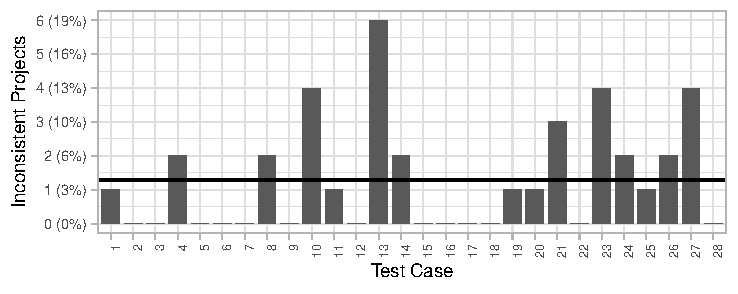
\includegraphics[width=\textwidth]{r/consistency-per-test-normal}%
        \vspace{-\medskipamount}
        \caption{Number of projects with inconsistent outcomes, per test case}
        \label{fig:consistency_per_test_normal}
    \end{subfigure}

    \bigskip

    \begin{subfigure}{.75\textwidth}
        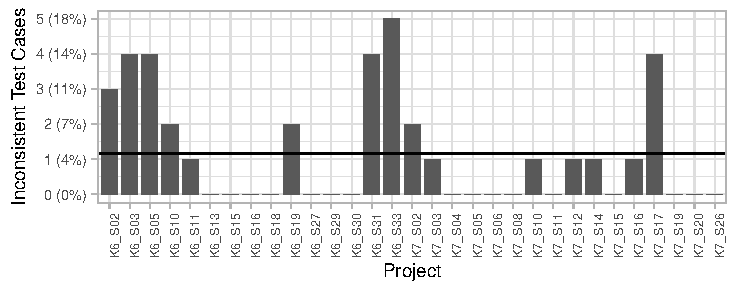
\includegraphics[width=\textwidth]{r/consistency-per-project-normal}%
        \vspace{-\medskipamount}
        \caption{Number of test cases with inconsistent outcomes, per project}
        \label{fig:consistency_per_project_normal}
    \end{subfigure}

    \caption{Inconsistent outcomes of test suite T1 over ten runs}
    \label{fig:consistency_normal}
\end{figure}

\begin{figure}[htpb]
    \centering
    \begin{subfigure}{.75\textwidth}
        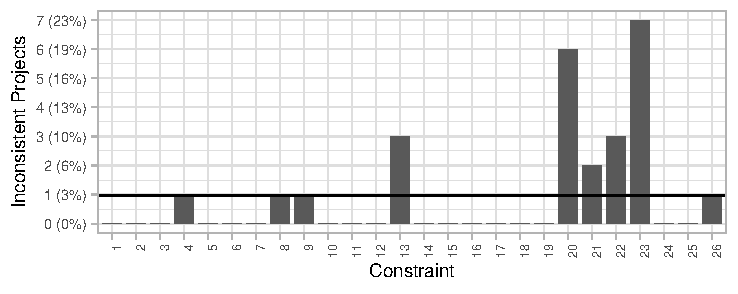
\includegraphics[width=\textwidth]{r/consistency-per-test-constraint}%
        \vspace{-\medskipamount}
        \caption{Number of projects with inconsistent outcomes, per constraint}
        \label{fig:consistency_per_test_constraint}
    \end{subfigure}

    \bigskip

    \begin{subfigure}{.75\textwidth}
        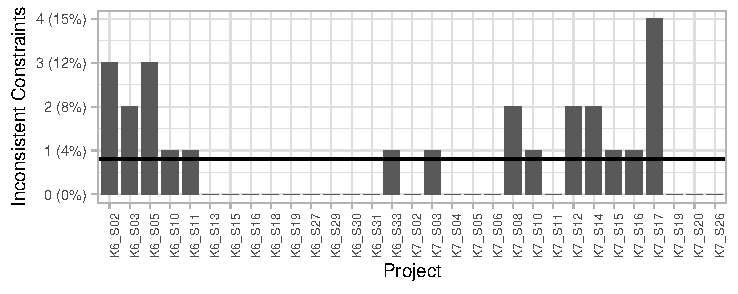
\includegraphics[width=\textwidth]{r/consistency-per-project-constraint}%
        \vspace{-\medskipamount}
        \caption{Number of constraints with inconsistent outcomes, per project}
        \label{fig:consistency_per_project_constraint}
    \end{subfigure}

    \caption{Inconsistent outcomes of test suite T2 over ten runs}
    \label{fig:consistency_constraint}
\end{figure}

\begin{figure}[htpb]
    \centering
    \begin{subfigure}{.75\textwidth}
        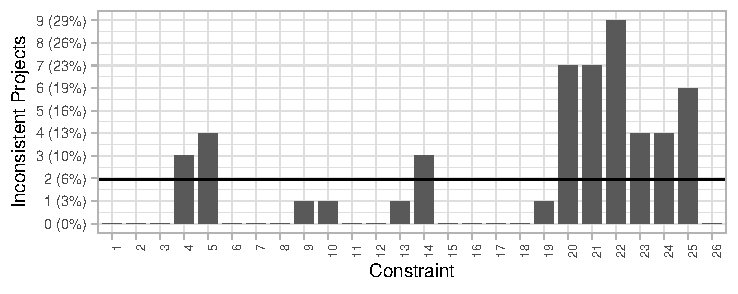
\includegraphics[width=\textwidth]{r/consistency-per-test-random}%
        \vspace{-\medskipamount}
        \caption{Number of projects with inconsistent outcomes, per constraint}
        \label{fig:consistency_per_test_random}
    \end{subfigure}

    \bigskip

    \begin{subfigure}{.75\textwidth}
        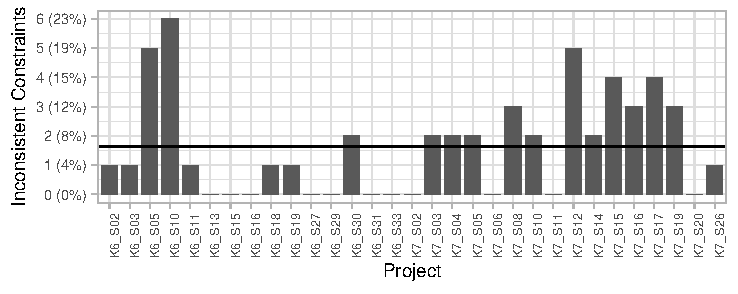
\includegraphics[width=\textwidth]{r/consistency-per-project-random}%
        \vspace{-\medskipamount}
        \caption{Number of constraints with inconsistent outcomes, per project}
        \label{fig:consistency_per_project_random}
    \end{subfigure}

    \caption{Inconsistent outcomes of test suite T3 over ten runs}
    \label{fig:consistency_random}
\end{figure}

\subsection{Causes for Inconsistent Test Outcomes}

% \mnote{In the discussion, write that Scratch programs tend to be inconsistent / non-deterministic because of their multimedia nature}
Inconsistent test outcomes can either be caused by the test case (or constraint) or by the project under test.
Therefore, we analyzed some of the inconsistencies of test suite T1 and their causes in Table~\ref{tab:inconsistencies_causes_normal}.
Most of them are caused by projects behaving in a non-deterministic manner,
tough some are caused by test cases themselves.
We noticed that tests, which deal with the banana sprite, i.e. test cases $13, 14, 23, 24, 25$, are relatively inconsistent.
We observed that the banana sprite is often poorly implemented, which causes it to behave inconsistently.
We suspect that students did not pay much attention to the banana sprite, since it is not essential to play the game.
A banana only subtracts points when it touches the ground, while an apple ends the game in this situation.
% Secondly, tests, which deal with the banana sprite are more likely to be inconsistent.
% In order to not go game over, tests have to periodically catch the falling apple with the bowl.
% This means, that the tests do not always, and are not always even able to, catch bananas with the bowl,
% which introduces inconsistency to tests, that rely on the behaviour of the banana.
\parspace

\begin{table}[htpb]
    \scalebox{0.95}{
    \scriptsize
    \begin{tabular}{lrlp{11.25cm}}
        \toprule
        Project & Test & Cause   & Description \\
        \midrule
        K6\_S11 & 1    & Both    & Test executes the program until each variable has been initialized to the correct value or until 500ms passed, and then checks the variable values.
                                   The project incorrectly increments the score variable continually when the program runs.
                                   Most of the time, the score variable has the value 0 when the rest of the program has been initialized,
                                   but sometimes the variable already gets incremented during initialization. \\
        K7\_S16 & 4    & Project & Program sometimes goes game over directly after being started. \\

        K6\_S03 & 8    & Project & Program moves banana to a random position on the ground when the right arrow key is pressed.
                                   Therefore the test has different outcomes depending on if the apple spawns left or right of the bowl. \\
        K6\_S33 & 8    & Both    & Test waits for 250ms to let the program initialize, then waits for a banana to appear at the top of the screen.
                                   K6\_S33 lets the banana fall instantly instead of waiting for a second (as specified),
                                   causing the banana to be below the tests threshold for detecting the banana ($y > 100$) after 250ms. \\

        K6\_S10 & 13   & Project & Program checks if the apple touches the ground with Scratch's "touching edge" primitive.
                                   Therefore, the program sometimes goes game over when an apple randomly spawns too much to the side of the screen and touches a vertical edge. \\
        K7\_S03 & 13   & Project & Program does not move banana to the top of the screen when it touches the ground, only when it touches the bowl.
                                   Therefore, the banana stays on the ground and is moved only when bowl moves over it, making banana re-spawns dependent on apple spawn locations. \\
        % K7\_S07 & 13   & Project & Test checks if a certain number of bananas spawn in 30 seconds.
        %                            Bananas fall very slowly in this project.
        %                            Because of this, enough bananas spawn if multiple bananas are randomly caught by the bowl,
        %                            but too few bananas spawn if bananas fall to the ground instead, because they have to travel more distance before they re-appear. \\

        % K6\_S02 & 14   & Project & Banana get stuck in the ground and only re-spawns if touched by the bowl. \\
        K6\_S10 & 14   & Test    & Test checks if bananas spawn at random x coordinates.
                                   The program uses clones for fruit sprites.
                                   The test detects the original sprite and the clone as two banana instances at the same x coordinate and concludes that bananas don't spawn at random x coordinatessthe same. \\
        K7\_S12 & 14   & Test    & Test failed because it detected two bananas spawning at the same x coordinate.
                                   In order to speed up test executions, we decided to wait for only two bananas to spawn and compare their positions.
                                   Therefore, while unlikely, it is possible that two bananas spawn in the same place by random chance, which fails the test. \\

        K7\_S17 & 19   & Project & Programs are supposed to check if the apple touches the color of the red stripe at the bottom to detect when the apple touches the ground.
                                   K7\_S17 checks for the wrong shade of red which is only present in some places, at the transition of the background and the red line.
                                   Therefore sprites are sometimes not detected touching the ground, and simply stay at the bottom of the screen. \\

        K6\_S05 & 20   & Project & To move the banana to a random position whenever it spawns,
                                   the program uses Scratch's builtin ''go to random position'', which moves it to a random y coordinate as well.
                                   Afterwards, it immediately adjusts the bananas y coordinate.
                                   But for a split second, the banana may touch the bowl or the ground without interaction, which the test detects. \\

        K7\_S02 & 21   & Both    & Program moves the apple to a random position on the ground 2 seconds after game over, causing the test to recognize it as not game over.
                                   The test could wait longer before performing checks to circumvent this problem. \\
        K7\_S10 & 21   & Project & Banana sometimes re-appears one more time after game over. \\
        % K6\_S10 & 23   & Test    & Test relies on the banana touching the bowl, but only follows the apple with the bowl in order to not go game over.
        %                            Therefore, sometimes the banana does not touch the bowl at all, resulting in a failing test. \\
        % K7\_S19 & 23   & Test    & The test checks if score is added when the apple touches the bowl.
        %                            It is skipped if the apple and the banana touch the bowl / ground in quick succession,
        %                            because the wrong score change might be considered, or the two score changes might happen in the same step. \\
        K6\_S19 & 23   & Test    & The test sometimes detects the banana touching the both the ground and the bowl as the it just touching the bowl. \\

        K6\_S02 & 27   & Both    & Banana can get stuck in the ground and continually subtract points for a short time after the time is up. \\
        K6\_S19 & 27   & Both    & Banana sometimes still falls for a short time after the time is up. \\
        K7\_S02 & 27   & Test    & Program never changes the score or time variable and has very slow falling apples.
                                   The test checks if the program went game over by checking that the variables and the sprites' x position does not change,
                                   but because the variables aren't changed and the apple falls very slowly, sometimes, the only thing that is changed is the sprites' y positions. \\
        \midrule
        K6\_S02 & 13   & Project & See K7\_S03, test 13. \\
        K6\_S03 & 13   & Project & See K6\_S03, test 8.  \\
        K7\_S17 & 21   & Project & See K7\_S17, test 19. \\
        K6\_S05 & 23   & Project & See K6\_S05, test 20. \\
        K7\_S17 & 23   & Test    & See K6\_S19, test 23. \\
        K6\_S05 & 24   & Project & See K6\_S05, test 20. \\
        K7\_S17 & 24   & Project & See K7\_S17, test 19. \\
        K6\_S05 & 25   & Project & See K6\_S05, test 20. \\
        \bottomrule
    \end{tabular}
    }
    \caption{Explanations for inconsistent outcomes of test suite T1}
    \label{tab:inconsistencies_causes_normal}
\end{table}

% current
%        1 2 3 4 5 6 7 8 9 1  11 12 13 14 15 16 17 18 19 20 21 22 23 24 25 26 27 28
% K6_S02                             1                                         1
% K6_S03               1             1
% K6_S05                                                  1        1  1  1
% K6_S10                             1  1
% K6_S11 1
% K6_S13
% K6_S15
% K6_S16
% K6_S18
% K6_S19                                                           1           1
% K6_S27
% K6_S29
% K6_S30
% K6_S31
% K6_S33               1
% K7_S02                                                     1                 1
% K7_S03                             1
% K7_S04
% K7_S05
% K7_S06
% K7_S08
% K7_S10                                                     1
% K7_S11
% K7_S12                                1
% K7_S14
% K7_S15
% K7_S16       1
% K7_S17                                               1     1     1  1
% K7_S19
% K7_S20
% K7_S26

% new
%        1 2 3 4 5 6 7 8 9 10 11 12 13 14 15 16 17 18 19 20 21 22 23 24 25 26 27 28
% K6_S02                    1        1                                         1
% K6_S03               1    1        1                                         1
% K6_S05                                                  1        1  1  1
% K6_S10                             1  1
% K6_S11 1
% K6_S13
% K6_S15
% K6_S16
% K6_S18
% K6_S19                                                           1           1
% K6_S27
% K6_S29
% K6_S30
% K6_S31                    1        1                             1        1
% K6_S33       1       1    1        1                                      1
% K7_S02                                                     1                 1
% K7_S03                             1
% K7_S04
% K7_S05
% K7_S06
% K7_S08
% K7_S10                                                     1
% K7_S11
% K7_S12                                1
% K7_S14                       1
% K7_S15
% K7_S16       1
% K7_S17                                               1     1     1  1
% K7_S19
% K7_S20
% K7_S26

\section{RQ3: Automated Input Generation}
\label{sec:rq3}

In this section, we will answer the following research question:

\begin{center}\begin{minipage}{.9\textwidth}
    \textbf{RQ3: What statement coverage can be achieved by controlling Scratch programs with automatically generated input?}
\end{minipage}\end{center}

\noindent For RQ1, we already showed that achieving accurate test results with random input is possible.
In order to get good test results generally, the generated input needs to be able to reach as much of the program under test as possible.
Intuitively, the more of a program gets executed, the more of the its functionality can be checked by tests running on it.
Therefore, we want to find out how much of typical Scratch programs' functionality can be reached by controlling it through Whisker's generated input.
In order to measure how much of the program is reached, we will use the achieved statement coverage as an indicator.
\parspace

We ran Whisker's automated input generation algorithm on each of the Code Club Scratch projects (P2) for ten minutes,
and measured the current statement coverage every second during the execution.
We chose not to reset the programs during the execution time,
since some of Code Club's projects require much execution time to be covered.
In fact, we also tried a configuration of ten minutes with four resets ($4 \times 2.5\text{min}$)
and got slightly worse results.
% Each program was run for five minutes and was reset five times during that time,
% resulting five one-minute executions of the program.
We use the mean final statement coverage on the projects to indicate how much of the programs is reached by the automated input.
To get more consistent results, we ran this experiment ten times, and took the average of the final coverage scores.
Listing~\ref{lst:coverage_test} shows the code, which we used to run the programs.
We chose to simulate random inputs with a duration between $100\text{ms}$ and $1000\text{ms}$ in an interval of $250\text{ms}$.
In order to access the coverage during the execution we implemented a function called \texttt{logCoverage},
which saves the current statement coverage of the program and outputs all saved coverage records once the test is over.
\parspace

% \mnote{TODO: remove?}
% \textbf{Correlation of test results and manual scoring.}
% Secondly, we want to determine how accurate results from tests with automatically generated input are.
% For this purpose, we tested the catching game projects (P1) with test suites T3 and T4,
% which are variations of the input-independent test suite T2, that uses Whisker's automated input generation to control the program.
% The catching game projects are especially challenging to be tested with automated input,
% since the catching game has a game over state, which is difficult to avoid.
% Like in RQ1, we use the correlation between test results and manual scores as an indicator of the test results' quality.
% \parspace

\begin{listing}[ht]
    \centering

    \begin{minipage}{.9\textwidth}
        \begin{javascriptcode}
            const measureCoverage = async function (t) {
                t.detectRandomInputs({duration: [100, 1000]});
                t.setRandomInputInterval(250);

                for (let timestamp = 1000; timestamp <= 600000; timestamp += 1000) {
                    await t.runUntil(() => t.getTotalTimeElapsed() >= timestamp);
                    t.logCoverage(timestamp, t.isProjectRunning());
                }
            }
        \end{javascriptcode}
    \end{minipage}

    \caption{Code to measure the coverage of automatically generated input}
    \label{lst:coverage_test}
\end{listing}

\noindent Figure~\ref{fig:coverage} shows the statement coverage we were able to achieve on the Code Club projects (P2)
with Whisker's automatically generated input on the first run,
as well as the execution time at which the coverage was achieved.
The black line in Figure~\ref{fig:coverage_line} displays the mean coverage of the projects.
After ten minutes of run time, we were able to achieve a mean coverage of $95.25\%$ with the lowest coverage for a project being $74\%$ and the highest being $100\%$.
We repeated this experiment ten times and got similar results, with the mean final coverage over ten runs being $95.25\%$.
The mean coverage from ten runs can be seen in Figure~\ref{fig:coverage_avg}.
In comparison, Figure~\ref{fig:coverage_no_input} and Figure~\ref{fig:coverage_no_input_avg} show the achieved coverage without simulating any inputs.
Here, we only got an average of $47.04\%$ per project on our first run, and $47.14\%$ averaged over ten runs.
\parspace

\begin{figure}[htpb]
    \centering
    \begin{subfigure}{.95\textwidth}
        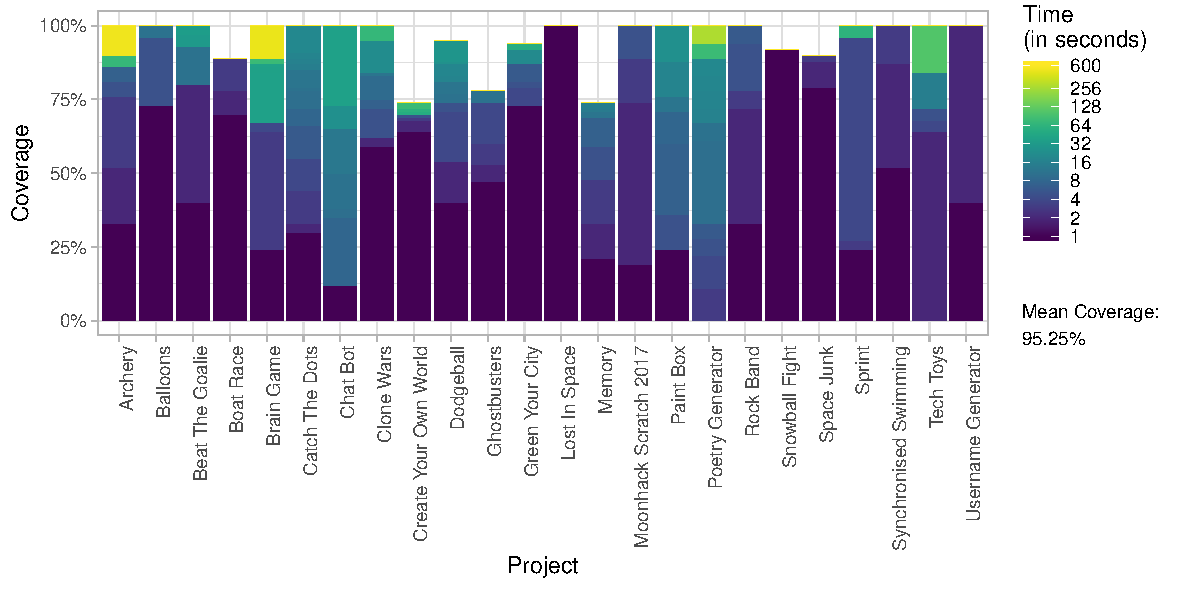
\includegraphics[width=\textwidth]{r/coverage-bar-random-input-1}
        \caption{Coverage per project}
        \label{fig:coverage_bar}
    \end{subfigure}

    \bigskip

    \begin{subfigure}{.95\textwidth}
        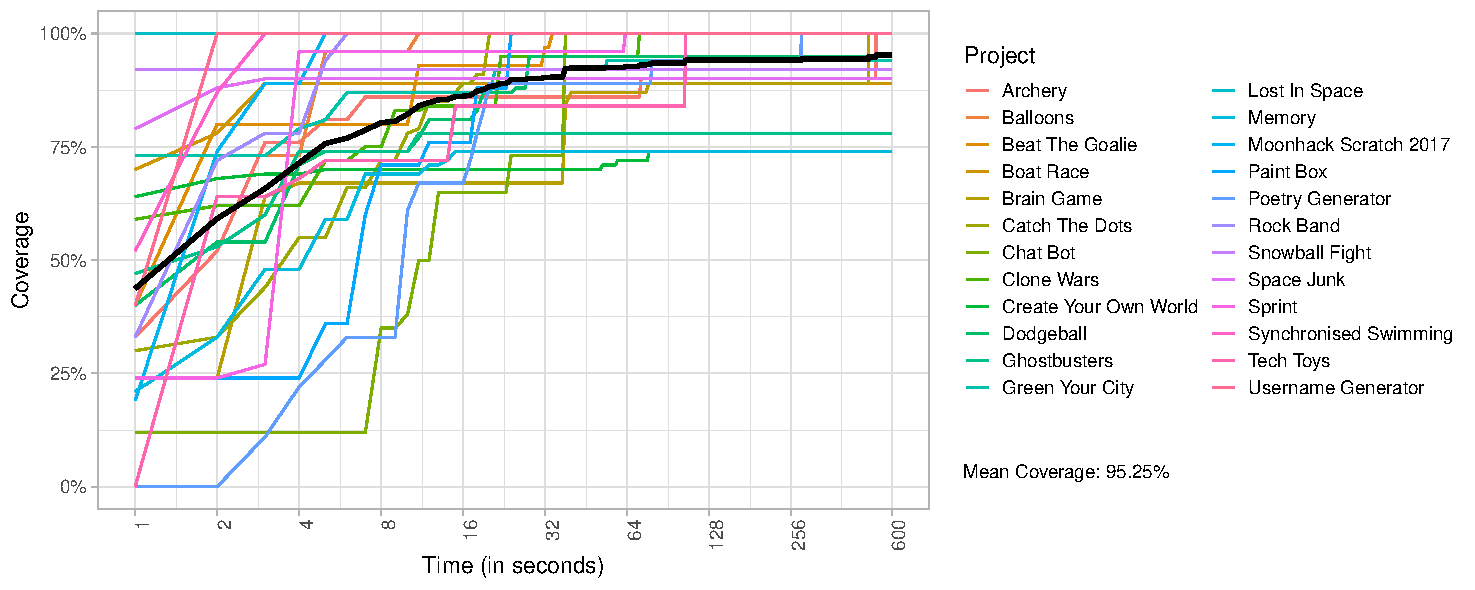
\includegraphics[width=\textwidth]{r/coverage-line-random-input-1}
        \caption{Coverage over time}
        \label{fig:coverage_line}
    \end{subfigure}

    \caption{Achieved coverage with automated input on the first run}
    \label{fig:coverage}
\end{figure}

\begin{figure}[htpb]
    \centering
    \begin{subfigure}{.95\textwidth}
        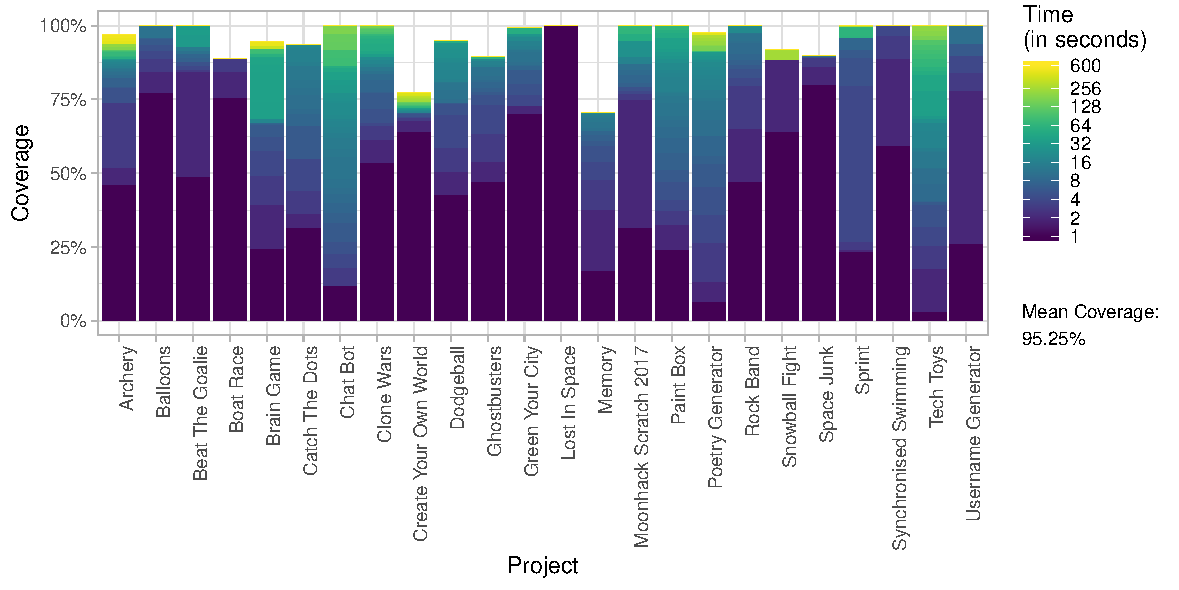
\includegraphics[width=\textwidth]{r/coverage-bar-random-input-avg}
        \caption{Coverage per project}
        \label{fig:coverage_bar_avg}
    \end{subfigure}

    \bigskip

    \begin{subfigure}{.95\textwidth}
        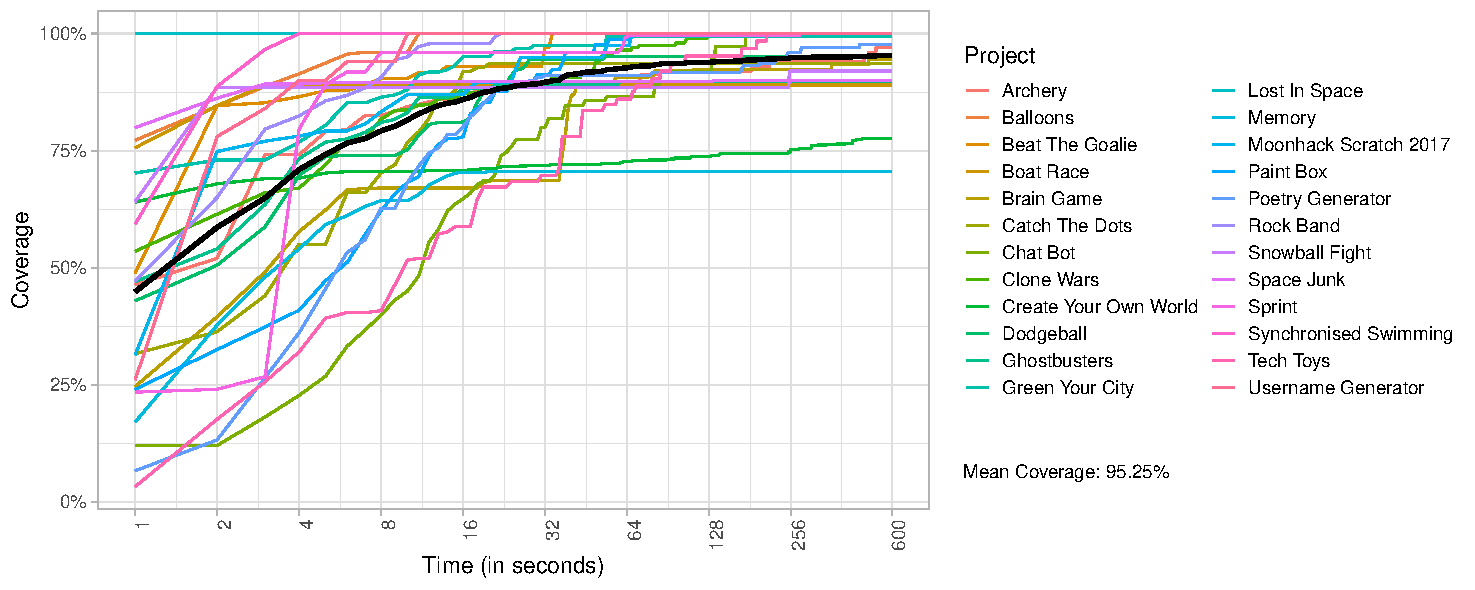
\includegraphics[width=\textwidth]{r/coverage-line-random-input-avg}
        \caption{Coverage over time}
        \label{fig:coverage_line_avg}
    \end{subfigure}

    \caption{Achieved coverage with automated input averaged over ten runs}
    \label{fig:coverage_avg}
\end{figure}

\begin{figure}[htpb]
    \centering
    \begin{subfigure}{.95\textwidth}
        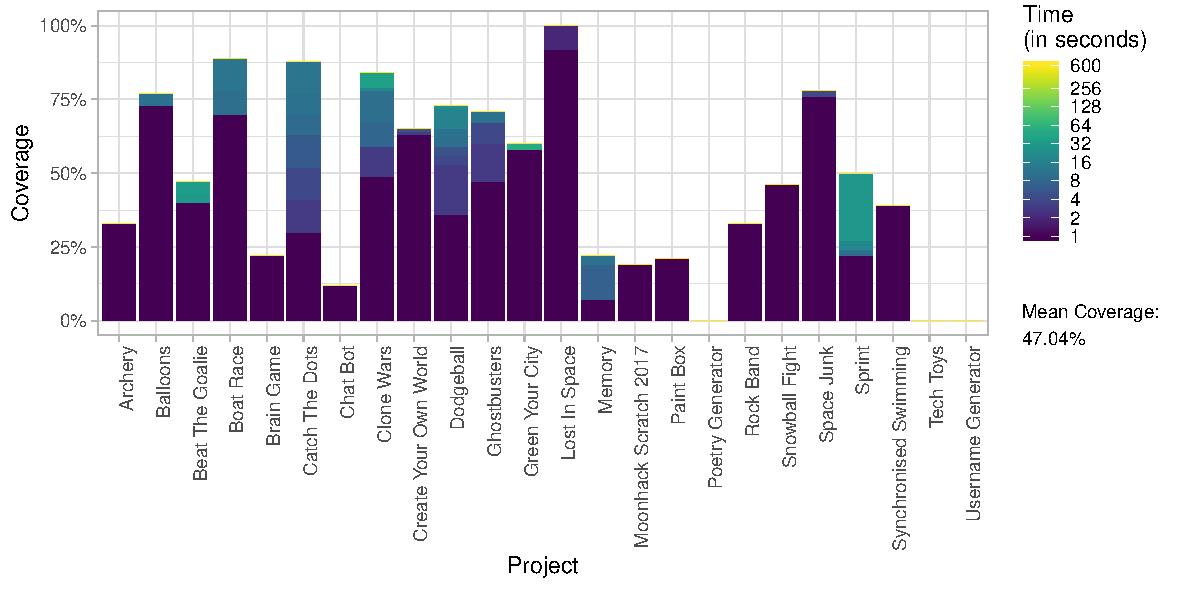
\includegraphics[width=\textwidth]{r/coverage-bar-no-input-1}
        \caption{Coverage per project}
        \label{fig:coverage_no_input_bar}
    \end{subfigure}

    \bigskip

    \begin{subfigure}{.95\textwidth}
        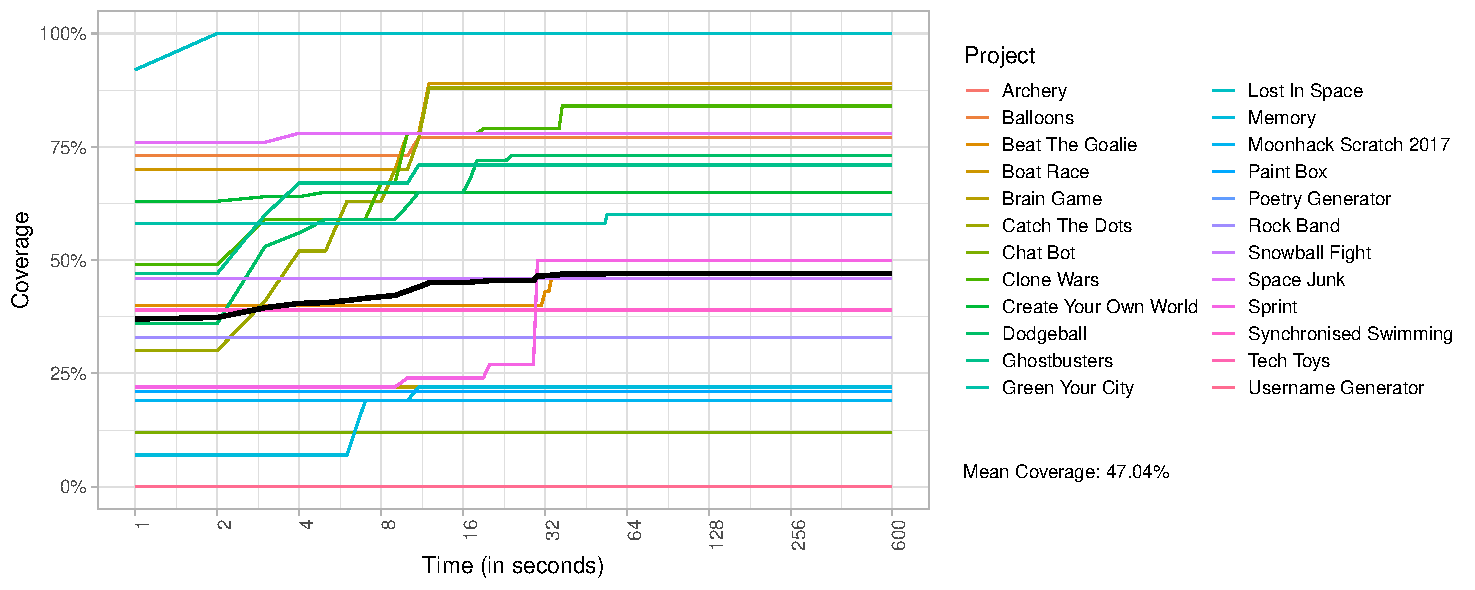
\includegraphics[width=\textwidth]{r/coverage-line-no-input-1}
        \caption{Coverage over time}
        \label{fig:coverage_no_input_line}
    \end{subfigure}

    \caption{Achieved coverage without input on the first run}
    \label{fig:coverage_no_input}
\end{figure}

\begin{figure}[htpb]
    \centering
    \begin{subfigure}{.95\textwidth}
        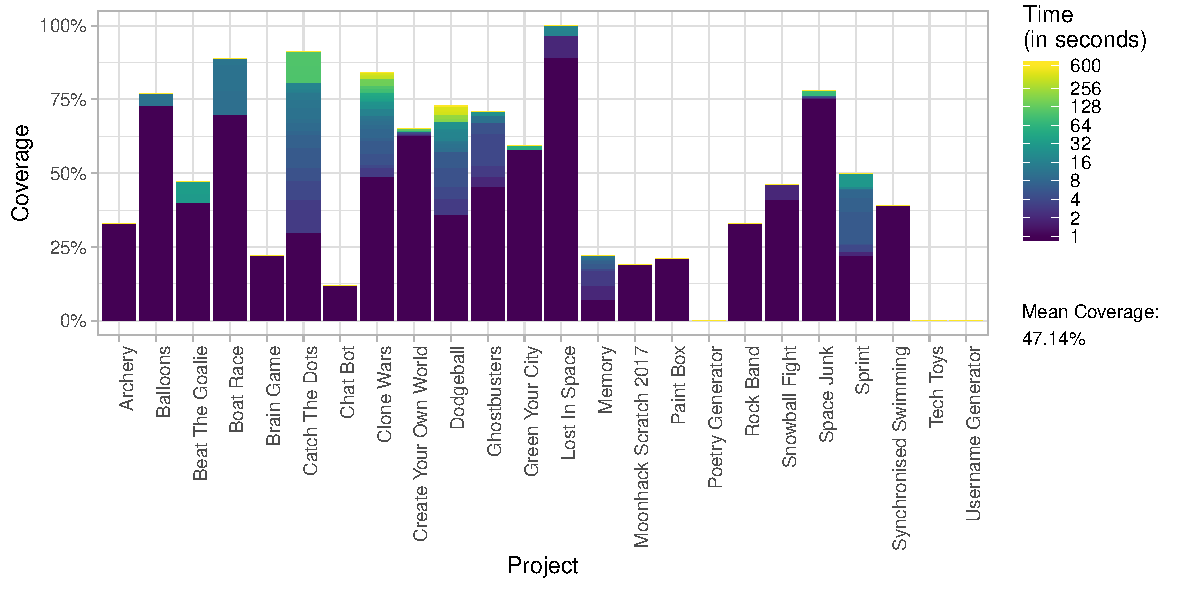
\includegraphics[width=\textwidth]{r/coverage-bar-no-input-avg}
        \caption{Coverage per project}
        \label{fig:coverage_no_input_bar_avg}
    \end{subfigure}

    \bigskip

    \begin{subfigure}{.95\textwidth}
        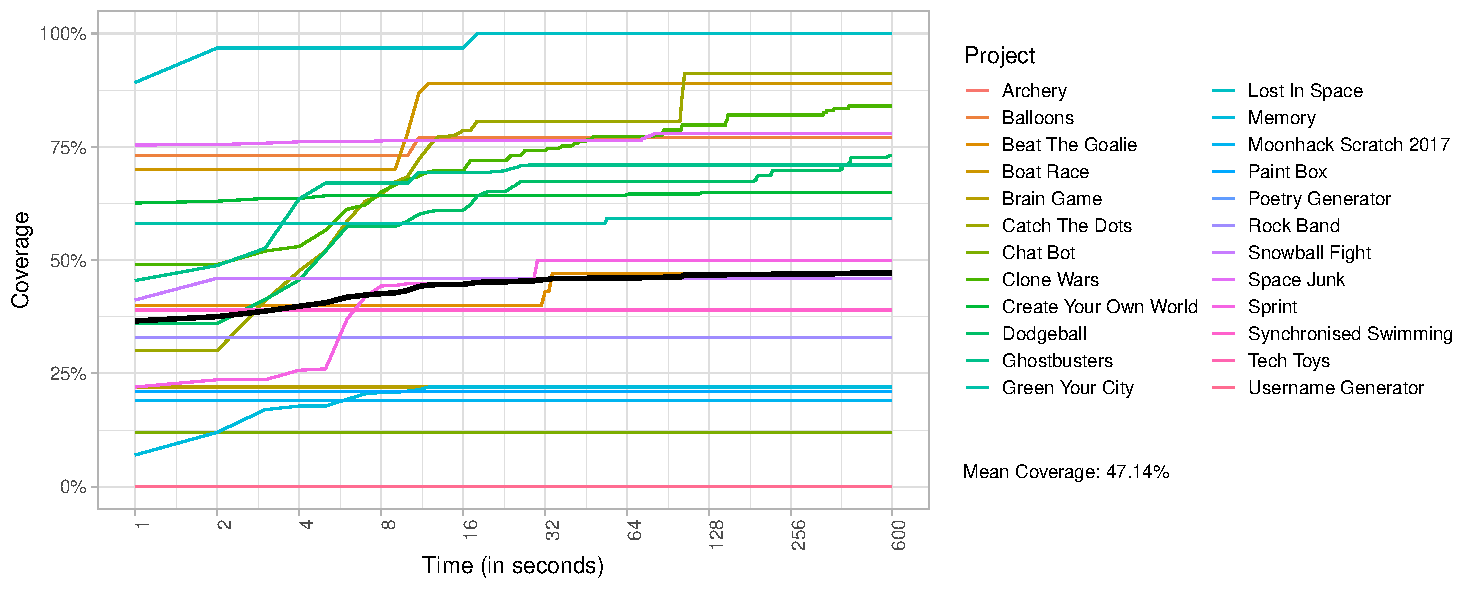
\includegraphics[width=\textwidth]{r/coverage-line-no-input-avg}
        \caption{Coverage over time}
        \label{fig:coverage_no_input_line_avg}
    \end{subfigure}

    \caption{Achieved coverage without input averaged over ten runs}
    \label{fig:coverage_no_input_avg}
\end{figure}

\subsection{Reasons for Low Coverage on Certain Projects}

Over the ten runs with generated input, we observed \textit{Create Your Own World} and \textit{Memory} consistently having the lowest coverage of the projects.
We are going to take a quick look at the reasons, why these projects are difficult to cover using random input.
A screenshot of both these programs can be seen in Figure~\ref{fig:difficult_code_club_projects}.

\begin{itemize}
    \item \textit{Create Your Own World} implements a little adventure game with a player sprite that is moved using the arrow keys.
        The player starts on the left of the screen and is able to move through several rooms using a portal on the right side of the screen.
        This project is difficult to cover, because the sprite needs to move a long way in one direction to reach a screen transition.
        But since each arrow key has equal probability to be simulated by Whisker, the sprite is more likely to only hover over a small area around its start position.
    \item In \textit{Memory} the player has to hit 4 different colored drums in an order that is randomly determined by the program.
        If the player hits one drum incorrectly, which includes hitting a drum while no order has been generated yet,
        the game goes into a game over state and can only be restarted by pressing the green flag.
        Therefore, using random inputs quickly results in an irrecoverable game over,
        because a wrong drum is hit, which renders much of the program's code unreachable.
\end{itemize}

\begin{figure}[htpb]
    \centering

    \begin{subfigure}{.3\textwidth}
        \centering
        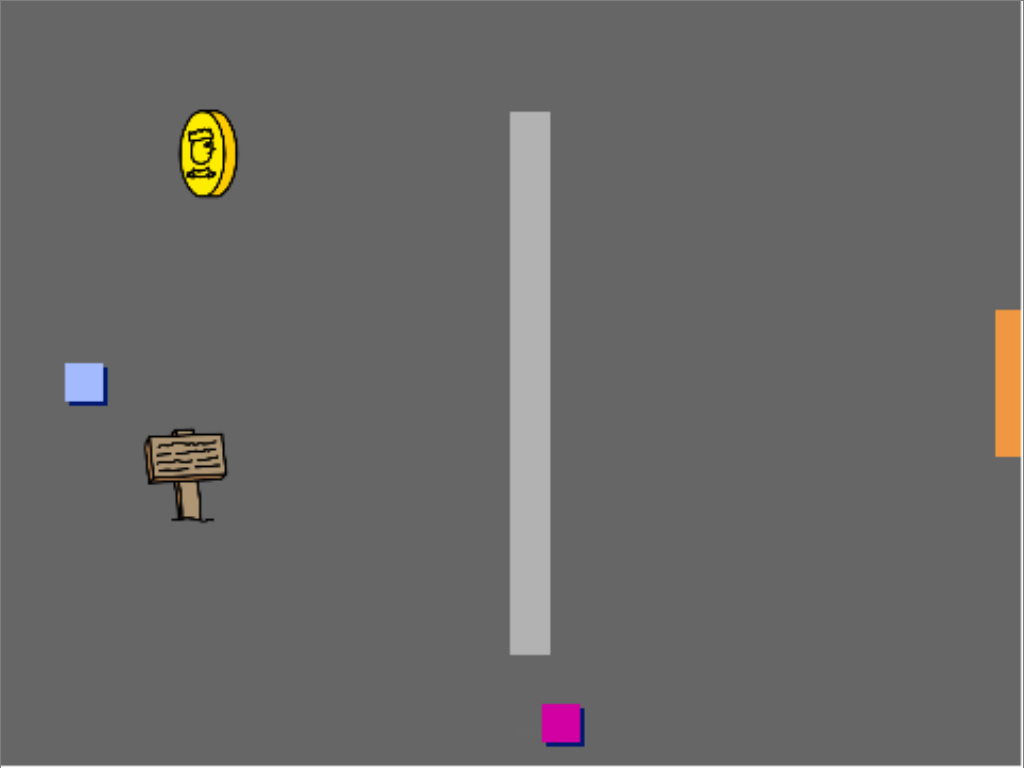
\includegraphics[width=\textwidth]{code-club-create-your-own-world}
        \caption{Create Your Own World}
    \end{subfigure}
    \hspace{1mm}
    \begin{subfigure}{.3\textwidth}
        \centering
        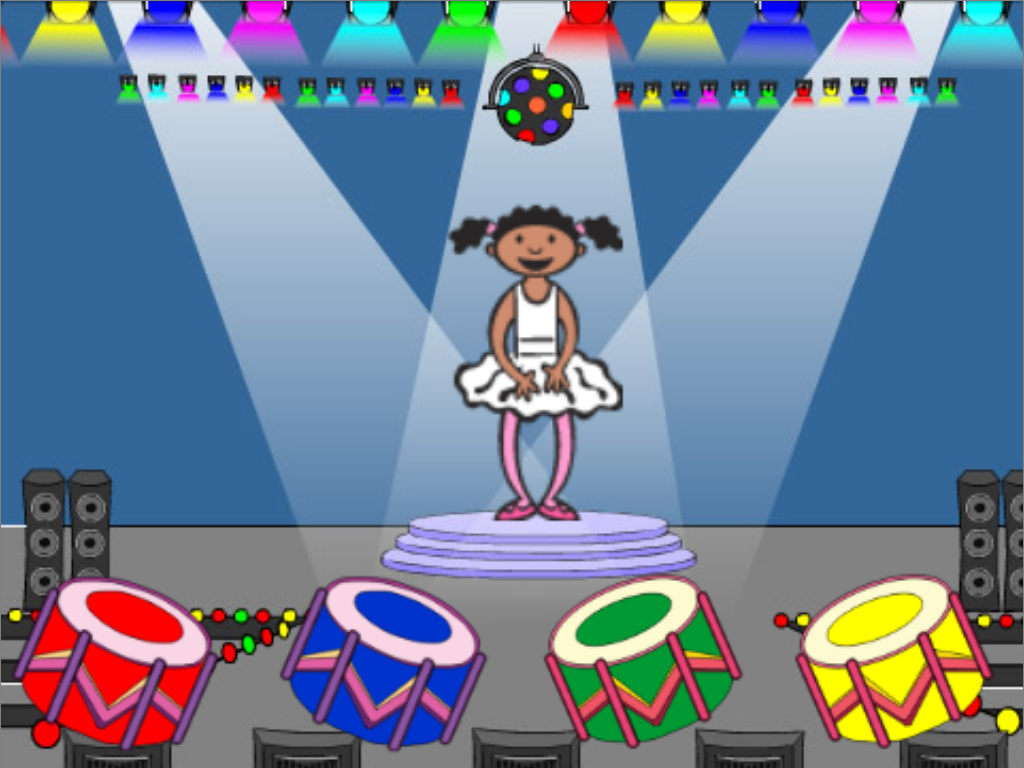
\includegraphics[width=\textwidth]{code-club-memory}
        \caption{Memory}
    \end{subfigure}%

    \caption{Screenshots of difficult to cover Code Club projects}
    \label{fig:difficult_code_club_projects}
\end{figure}

\section{RQ4: Interference with Programs Under Test}
\label{sec:rq4}

In this section, we will answer the following research question:

\begin{center}\begin{minipage}{.9\textwidth}
    \textbf{RQ4: Does the testing process slow down the program under test?}
\end{minipage}\end{center}

\noindent Since JavaScript is executed in a single-threaded environment,
Whisker executing code in between steps of the Scratch program can possibly delay execution steps of the program.
This can be problematic because some of Scratch's blocks,
specifically the \texttt{wait} blocks, depend on real time.
Therefore, executing additional code could influence time-related behaviour of the program,
although we suspect that this will not be a concern for most Scratch programs.
\parspace

Scratch's step function has to be called 30 times per second.
Therefore, the execution time of Whisker's step procedure, which includes the execution of Scratch's step,
should not exceed $1000\text{ms} \div 30 = 33.33\text{ms}$.
Scratch allocates $0.75 \times 33.33\text{ms} = 25.0\text{ms}$ of the $33.33\text{ms}$ to execute the program.
If no sprite changes occur during the step,
the Scratch VM will execute the program for the allocated amount of time.
But if some sprite's position or appearance changes, the VM will stop executing the program earlier.
Afterwards, Scratch draws the new frame in the GUI.
In the worst case, i.e. if no sprite changes and the whole time interval is used to execute the program,
$0.25 * 33.33\text{ms} = 8.33\text{ms}$ will be left to render the new frame.
Most modern hardware will take significantly less time than $8.33\text{ms}$ to render the picture,
which leaves time for Whisker to execute other tasks.
\parspace

We should also note that coverage measurement gets done during Scratch's step,
which will slow the program down if the full $25\text{ms}$ of execution time are used.
However the Scratch GUI also registers code to update the user interface, which is run during the step of the VM,
so this should not affect the program any more than Scratch's GUI itself does.
Callbacks for sprite changes, i.e. \texttt{onSpriteMoved} and \texttt{onSpriteVisualChange},
are also executed during Scratch's step, but if one of these functions is executed, a redraw request will be issued anyways,
causing the step execution to end earlier.
\parspace

To evaluate this,
we executed our test suites T1-T3 on the sample solution of the catching game (P1) ten times,
and measured the execution time of Whisker's components (see Figure~\ref{fig:whisker_step_procedure})
as well as the execution time of Scratch during each step.
Since we executed Whisker in a web browser,
we were limited to JavaScript's \texttt{performance.now} method to measure execution times,
which has an accuracy of $0.1\text{ms}$.
The code we used for measuring the execution times can be found in Listing~\ref{lst:time_measurement_code} in the appendix.
We will consider the mean execution times, as well as the maximum execution times from the ten runs
to decide if the tests could interfere with the program.

\clearpage

\paragraph{Null hypothesis ($H_0$):}
The execution of additional code delays the execution of Scratch's steps, which possibly interferes with the program execution.
\vspace{-\medskipamount}
\paragraph{Alternative hypothesis ($H_1$):}
The execution of additional code introduces no delay. It will therefore not interfere with the program execution.
\parspace

\noindent Figure \ref{fig:time_line_plot} shows the total execution times
from the first run of each test suite on the sample program.
The time measurements include both the execution time of Whisker and Scratch.
We can see that the execution time is mostly far beneath the limit of $33.33\text{ms}$
and only rarely spikes to higher for short periods of time.
\parspace

\begin{figure}[htpb]
    \centering

    \begin{subfigure}{\textwidth}
        \centering
        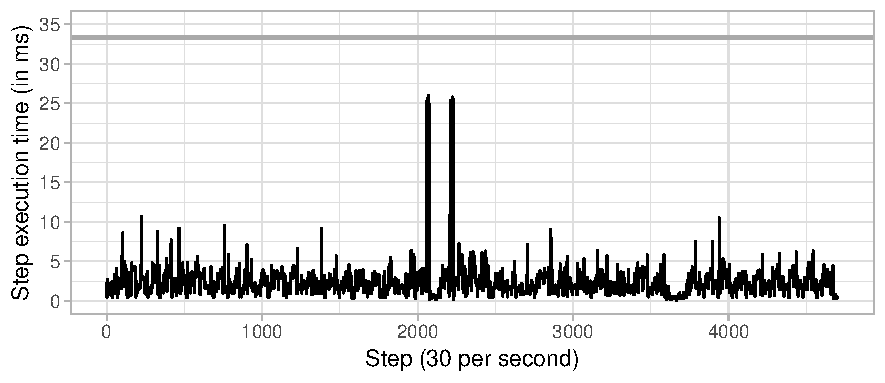
\includegraphics[width=.7\textwidth]{r/time-normal}
        \vspace{-\medskipamount}
        \caption{Time measurements for test suite T1 (normal)}
    \end{subfigure}

    \bigskip

    \begin{subfigure}{\textwidth}
        \centering
        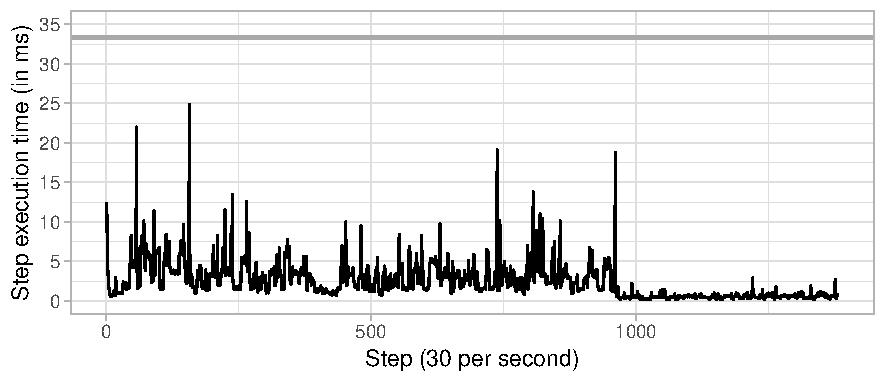
\includegraphics[width=.7\textwidth]{r/time-constraint}
        \vspace{-\medskipamount}
        \caption{Time measurements for test suite T2 (constraint)}
    \end{subfigure}

    \bigskip

    \begin{subfigure}{\textwidth}
        \centering
        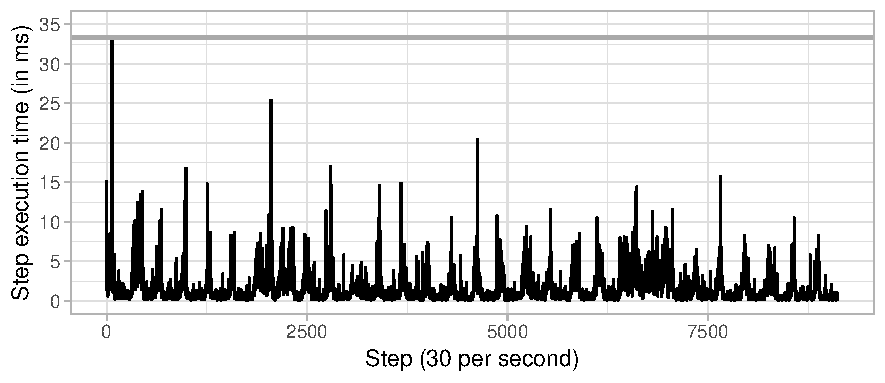
\includegraphics[width=.7\textwidth]{r/time-random}
        \vspace{-\medskipamount}
        \caption{Time measurements for test suite T3 (random input)}
    \end{subfigure}

    \caption{Measured execution times of Whisker's step procedure (in ms) during the first test execution}
    \label{fig:time_line_plot}
\end{figure}

\clearpage

Table \ref{tab:time_measurements} shows the mean and the maximum of execution times for each part of Whisker's step procedure.
This data is taken from ten consecutive executions of each test suite on the program under test.
The average total step execution time is far beneath $33.33\text{ms}$ with $1.972\text{ms}$, $2.272\text{ms}$ and $1.330\text{ms}$ for test suites T1-T3 respectively.
The maximum total step execution times were $35.1\text{ms}$, $24.9\text{ms}$ and $33.1\text{ms}$.
We can observe that the execution of test suite T1 spiked over the $33.33\text{ms}$ with a maximum of $35.1\text{ms}$,
but this only happened in one single step, with the second longest step execution time for T1 being $31.1\text{ms}$.

% round((0.071 + 0.102 + 0.068) / 3, digits = 3)
% round((0.004 + 0.004 + 0.024) / 3, digits = 3)
% round((0.005 + 0.005 + 0.023) / 3, digits = 3)
% round((0.022 + 0.022 + 0.022) / 3, digits = 3)
% round((1.852 + 2.054 + 1.129) / 3, digits = 3)
% round((0.007 + 0.006 + 0.005) / 3, digits = 3)
% round((0.012 + 0.078 + 0.058) / 3, digits = 3)
% round((1.972 + 2.272 + 1.330) / 3, digits = 3)
% round((0.12  + 0.218 + 0.201) / 3, digits = 3)
%
% round(max(4.8  , 7.3  , 9.7 ), digits=3)
% round(max(1.3  , 3.1  , 6.4 ), digits=3)
% round(max(2    , 1.6  , 8.6 ), digits=3)
% round(max(6.4  , 4.2  , 4.8 ), digits=3)
% round(max(35.1 , 24.6 , 32.7), digits=3)
% round(max(1.1  , 0.3  , 1.8 ), digits=3)
% round(max(2.9  , 3.2  , 12.5), digits=3)
% round(max(35.1 , 24.9 , 33.1), digits=3)
% round(max(6.5  , 7.6  , 13.1), digits=3)

\begin{table}[htpb]
    \centering
    \footnotesize
    \begin{tabular}{l|rr|rr|rr}
        \toprule
                                     &       & T1   &       & T2   &       & T3   \\
                                     & mean  & max  & mean  & max  & mean  & max  \\
        \midrule
        Callbacks (Before)           & 0.071 & 4.8  & 0.102 & 7.3  & 0.068 & 9.7  \\
        Random Inputs                & 0.004 & 1.3  & 0.004 & 3.1  & 0.024 & 6.4  \\
        Inputs                       & 0.005 & 2.0  & 0.005 & 1.6  & 0.023 & 8.6  \\
        Sprites                      & 0.022 & 6.4  & 0.022 & 4.2  & 0.022 & 4.8  \\
        Scratch (Program + Renderer) & 1.852 & 35.1 & 2.054 & 24.6 & 1.129 & 32.7 \\
        Callbacks (After)            & 0.007 & 1.1  & 0.006 & 0.3  & 0.005 & 1.8  \\
        Constraints                  & 0.012 & 2.9  & 0.078 & 3.2  & 0.058 & 12.5 \\
        \midrule
        Total                        & 1.972 & 35.1 & 2.272 & 24.9 & 1.330 & 33.1 \\
        Total (Whisker only)         & 0.12  & 6.5  & 0.218 & 7.6  & 0.201 & 13.1 \\
        \bottomrule
    \end{tabular}
    \caption{Measured execution time (in ms) for every part of Whisker's step procedure over ten test executions}
    \label{tab:time_measurements}
\end{table}

\section{Discussion}
\label{sec:discussion}

In this evaluation, we conducted three separate experiments to examine the usefulness of Whisker.
In the first experiment, we analyzed test results of three different test suites.
We found out, that all of the results consistently show a strong correlation to independent manual scores.
Therefore, we reject the null hypothesis of RQ1.
We also proved that the constraint testing approach is able to deliver accurate test results,
both with deliberate input and with automatically generated input.
\parspace

We analyzed the flakiness of the test suites and measured a percentage of $4.15\%$ inconsistent project-test combinations for test suite T1,
$3.10\%$ for test suite T2, and $6.32\%$ for test suite T3.
We found several reasons why certain tests and certain programs can be flaky.
Many inconsistent results were caused by non-deterministic behaviour of the programs under test,
which may be counteracted in the future by seeding Scratch's random number generator.
% We suspect that simpler programs can be tested with much fewer inconsistencies.
At the same time, more experience in automated testing for Scratch will lead to more robust and less flaky test suites.
The test suites we used were written early during development of Whisker.
Therefore, the test suites had some more or less obvious flaws,
some of which can be seen in Table~\ref{tab:inconsistencies_causes_normal} from the flakiness evaluation.
And of course, tests that involve randomly generated input show a higher number of inconsistent outcomes,
since the tests themselves are non-deterministic.
\parspace

The second experiment dealt with automated input generation.
We let Whisker's automated input generation algorithm run on several Scratch programs ten times,
then we ran the same programs without any input.
We measured the achieved statement coverage on the programs during both executions,
and compared their averages.
% Since the automated input was able to achieve much higher coverage than running the programs without simulating input,
% we rejected the null hypothesis.
The mean statement coverage amounted to $95.25\%$ with automated input, and $47.14\%$ without input.
This shows that simple randomly generated input is able to reach much of typical Scratch programs' functionality.
\parspace

Finally, we conducted another experiment to find out
if the testing process would slow down the program under test.
For this purpose, we measured the execution time of Whisker's step procedure on the execution of our test suites.
We found that Scratch's allocated time interval for computations is long enough to
allow executing both the Scratch program and test code.
Sometimes, the execution time of the step procedure spiked over the allocated time interval,
delaying a single step.
However, these single spikes should not affect the programs in a meaningful way.
The execution times will only be problematic if they consistently exceed the time limit.
Therefore, programs under test were not affected by Whisker in our tests, and we can reject the null hypothesis of RQ4.


\section{Threats to Validity}
\label{sec:threats_to_validity}

As is usual, the empirical studies we conducted in this work must confront certain threats to validity.
Possible threats fall into one of two categories.
On the one hand, threats to internal validity represent factors which provide alternative explanations for the presented results.
On the other hand, threats to external validity deal with the generalizability of the results.

\subsection{Internal validity}

Conditions which could influence any test outcomes, correlations, coverage measurements,
or time measurements are possible threads to internal validity.
\parspace

\textbf{Independence of ground truth.}
One threat to validity arises from the use of the manually assigned scores as
ground truth to assess the quality of test results.
If we assigned the scores ourselves,
a comparison to them would not be adequate to give evidence about the quality of the results.
However, the manual scores were assigned by the teacher after the course was held,
and tests were written independently of the grading scheme, only using the textual specification of the program.
Therefore, the manual scores are completely independent from our test results,
and a comparison between the two is adequate.
\parspace

\textbf{Randomness.}
Another threat is, of course, random chance.
Many Scratch programs use randomness, which can make test outcomes inconsistent.
To eliminate the possibility of random chance affecting our test results as much as possible, we executed each test suite ten times,
and considered the average results in addition to results from single executions.
\parspace

\textbf{RAM usage.}
% Another possible threat comes from the execution order of the programs.
One more possible threat comes from an issue of Scratch itself.
At the time of the evaluation, Scratch had a problem of consuming increasing amounts of memory when loading many programs in succession,
which, in theory, could have interfered with the execution of our test suites.
However, we payed close attention to the RAM usage of the machine that executed the tests.
We also performed some of our test suite executions on all projects sequentially,
and some on one half of the programs, then later on the other half.
We observed similar results with both methods, therefore this issue did not have any impact on our test results.
% This could be problematic if we executed the programs in order of descending manual scores.
% However, we executed each test suite on the projects in alphabetical order,
% and the manual scores actually show a weak positive correlation ($r = 0.43$) to the indexes of the execution order,
% meaning that the alphabetical order is closer to the order of ascending manual scores.
\parspace

\textbf{Excluded Projects.}
For RQ1, we excluded multiple Scratch projects from our statistics because they had various problems that
would create a discrepancy between test results and manual scoring due to differences in the scoring methods.
For the most part, these projects could not be started correctly,
either because they did not use the green flag or because the projects were missing initialization and were
saved in a state that causes an early game over.
We conjecture that programs which were written with automated testing in mind won't have this kind of problems.
If students are given a way to perform the tests on their program themselves, they will realize that the program is not starting correctly.
And in most cases these problems are fairly easy to solve.
Therefore, we believe that the statistics show more realistic results with these projects excluded.

\subsection{External Validity}

Factors which limit the generalizability of the results in this work are possible threats to external validity.
\parspace

\textbf{Programs under test.} For one thing, the program under test could be chosen poorly,
making the results not applicable for other Scratch programs.
Therefore, we tried to choose programs that are representative of Whisker's target usage in the field of education.
We chose Scratch projects from an actual workshop for students.
The program has user interaction, uses randomness, and has a game over state,
which are all important challenges for testing Scratch programs.
To evaluate the automated input generation,
we again went with programs from Scratch courses.
The programs feature many different input methods and interactions,
which make them suitable to evaluate automated input on.
\parspace

\textbf{Tests for time measurements.}
To find out if Whisker would slow down programs under test,
we executed our test suites and measured the execution times of Whisker's step procedure.
One could argue that the execution times can be raised by a variety factors.
More, as well as more computationally expensive, callbacks and constraints can be registered,
more random inputs can be registered,
and a Scratch program with more sprites can be chosen.
Therefore, tests suites can interfere with the program under test, if they do it purposefully.
However, we wanted to measure the execution time of a realistic test suite on a realistic program.
This setup did not change the program's behaviour,
and the measurements indicate that more expensive test suites will still be fine as well.
% \parspace
%
% \textbf{Hardware for time measurements.}
% Since the measurements of step execution times depend on the used hardware,
% it is important to use a realistic testing environment for that purpose.
% Therefore, we did not only perform measurements on the main computer we used for other experiments,
% but also on a less powerful laptop, which we suspect is a more realistic hardware configuration for Whisker.
